\documentclass[11pt, twocolumn]{report}
\usepackage[a4paper, hmargin={2.8cm, 2.8cm}, vmargin={2.5cm, 2.5cm}]{geometry}
%\usepackage[T1]{fontenc}
\usepackage[utf8]{inputenc}
\usepackage{eso-pic} % \AddToShipoutPicture
\usepackage{graphicx} % \includegraphics
\usepackage[english]{babel}
\usepackage{tcolorbox}
\usepackage{multicol}
\usepackage{amssymb}
\usepackage{amsmath}
\usepackage{fancyhdr}
\usepackage{fancyvrb}
\usepackage{geometry}
\usepackage{listings}
\usepackage[hyphens]{url}
\usepackage{breakurl}
\usepackage{cite}
\usepackage{color}
\usepackage{svg}
\usepackage{makecell}
\usepackage{array}
\usepackage{multicol}
\usepackage{subcaption}
\usepackage[toc,page]{appendix}
\usepackage[breaklinks=true,pdfusetitle]{hyperref}
\usepackage{float}
\usepackage{xcolor}
\usepackage{tablefootnote}
\usepackage{footnote}
\usepackage{lipsum}
\usepackage{tocloft}
\usepackage{blindtext}
\usepackage{enumitem}
\usepackage{minted}
\usepackage{algorithm}
\usepackage{algpseudocode}
\usepackage{subcaption}
\usepackage{pbox}
\usepackage{glossaries}
\usepackage{xargs}
\usepackage[colorinlistoftodos,prependcaption,textsize=tiny]{todonotes}
\newacronym{sme}{SME}{Synchronous Message Exchange}
\newacronym{arp}{ARP}{Address Resolution Protocol}
\newacronym{ip}{IP}{Internet Protocol}
\newacronym{dhcp}{DHCP}{Dynamic Host Configuration Protocol}
\newacronym{ipv4}{IPv4}{Internet Protocol version 4}
\newacronym{ipv6}{IPv6}{Internet Protocol version 6}
\newacronym{nic}{NIC}{Network Interface Controller}
\newacronym{csp}{CSP}{Communicating Sequential Processes}
\newacronym{gpl}{GPL}{General Purpose Language}
\newacronym{tcp}{TCP}{Transmission Control Protocol}
\newacronym{udp}{UDP}{User Datagram Protocol}
\newacronym{dsl}{DSL}{Domain-specific Language}
\newacronym{vhsic}{VHSIC}{Very High Speed Integrated Circuit}
\newacronym{vhdl}{VHDL}{\acrshort{vhsic} Hardware Description Language}
\newacronym{hdl}{HDL}{Hardware Description Language}
\newacronym{smeil}{SMEIL}{SME Implementation Language}
\newacronym{il}{IL}{Intermediate Language}
\newacronym{axi}{AXI}{Advanced eXtensible Interface}
\newacronym{hls}{HLS}{High-Level Synthesis}
\newacronym{gpgpu}{GPGPU}{General Purpose Graphics Processing Unit}
\newacronym{cpu}{CPU}{Central Processing Unit}
\newacronym{fpga}{FPGA}{Field-Programmable Gate Array}
\newacronym{ic}{IC}{Integrated Circuit}
\newacronym{asic}{ASIC}{Application Specific Integrated Circuit}
\newacronym{bp}{BP}{Buffer-Producer}
\newacronym{cp}{CP}{Compute-Producer}
\newacronym{toe}{TOE}{TCP offload engine}
\newacronym{icmp}{ICMP}{Internet Control Message Protocol}
\newacronym{rtl}{RTL}{Register-transfer level}
\newacronym{cpld}{CPLD}{Complex Programmable Logic Device}
\newacronym{soc}{SoC}{System on a Chip}
\newacronym{smtp}{SMTP}{Simple Mail Transfer Protocol}
\newacronym{ftp}{FTP}{File Transfer Protocol}
\newacronym{http}{HTTP}{HyperText Transfer Protocol}
\newacronym{slip}{SLIP}{Serial Line Internet Protocol}
\newacronym{ppp}{PPP}{Point-to-Point Protocol}
\newacronym{fddi}{FDDI}{Fiber Distributed Data Interface}
\newacronym{ieee}{IEEE}{Institute of Electrical and Electronics Engineers}
\newacronym{tos}{ToS}{Type of Service}
\newacronym{ttl}{TTL}{Time To Live}
\newacronym{alu}{ALU}{Arithmetic Logic Unit}
\newacronym{eeprom}{EEPROM}{Electrically Erasable Programmable Read-Only Memory}
\newacronym{voip}{VoIP}{Voice over IP}
\newacronym{dos attack}{DoS attack}{Denial-of-Service attack}
\newacronym{iot}{IoT}{Internet of things}
\newacronym{fifo}{FIFO}{First In, First Out}
\newacronym{www}{WWW}{World Wide Web}
\newacronym{ssh}{SSH}{Secure Shell}
\newacronym{p2p}{P2P}{Peer-to-Peer}












% \newacronym{}{}{}









\makeglossaries

%Footnote setup
%\counterwithout*{footnote}{chapter}

%Hyperref setup
\pdfstringdefDisableCommands{%
  \let\vspace\@gobble
}

%\usepackage{coffee4} % Comment me out
% minted styles
%\newmintinline['mintedinlineitem']{csharp}{breaklines}
%\setmintedinline{breaklines}
\setminted[csharp]{escapeinside={*@}{@*}}
\newmintinline[csharpextend]{minted-lexers/csharp.py:MDCSharpLexer -x}{breaklines}

% Define Listings
\definecolor{codegreen}{rgb}{0,0.6,0}
\definecolor{codegray}{rgb}{0.5,0.5,0.5}
\definecolor{codepurple}{rgb}{0.58,0,0.82}
\definecolor{codeblue}{rgb}{0,0,0.95}
\definecolor{backcolour}{rgb}{0.95,0.95,0.95}

\lstdefinestyle{sme}{
    backgroundcolor=\color{backcolour},
    commentstyle=\color{codegreen},
    keywordstyle=\color{codeblue},
    numberstyle=\tiny\color{codegray},
    stringstyle=\color{codeblue},
    basicstyle=\ttfamily\footnotesize,
    xleftmargin=15pt,
    framexleftmargin=15pt,
    framexrightmargin=2pt,
    framexbottommargin=2pt,
    frame=single,
    breakatwhitespace=false,
    breaklines=true,
    breakatwhitespace=true, % Do not break at "other" characters
    captionpos=b,
    keepspaces=true,
    numbers=left,
    numbersep=5pt,
    showspaces=false,
    showstringspaces=false,
    showtabs=false,
    tabsize=2,
}

\lstset{style=sme}


%%% Macros
% easier figure
% usage: \pic{width}{image}{caption}{label}
\newcommand\pic[4]{% these comment signs will prevent the introduction of spurious spaces
  \begin{figure}[h!]
  \centering
  \includegraphics[width=#1\textwidth]{#2}
  \caption{#3}
  \label{#4}
  \end{figure}
}




\newcolumntype{C}[1]{>{\centering\let\newline\\\arraybackslash\hspace{0pt}}m{#1}}
\setlength{\columnsep}{1cm}
\newcommand*\tablerot{\rotatebox{90}}


\author{%
Meznik, Jan\\%
\texttt{pzj895@alumni.ku.dk}\\%
\texttt{jan@meznik.dk}%
\and%
Jacobi, Mark Jan\\%
\texttt{dcz738@alumni.ku.dk}\\%
\texttt{mark@jacobi.pm}%
}

\title{%
\vspace{3cm}%
\huge{TCP/IP in hardware using SME}\\
\vspace{0.5cm}%
%	\Large{Write something clever here}
}



% Header
\pagestyle{fancy}


\iffalse
\fancyhf{}
%\fancyhead[L]{}
%\fancyhead[R]{}
%\fancyhead[C]{}
%\fancyfoot[C]{Center \leftmark}
\fi

\lhead{University of Copenhagen}
%\chead{}
\rhead{TCP/IP in SME}


\begin{document}
\onecolumn


%%%%% KU HEADER %%%%%%%%%%%%%%%%%%%%%%%
\AddToShipoutPicture*{\put(0,0){\includegraphics*[viewport=0 0 700 600]{include/natbio-farve}}}
\AddToShipoutPicture*{\put(0,602){\includegraphics*[viewport=0 600 700 1600]{include/natbio-farve}}}
\AddToShipoutPicture*{\put(0,0){\includegraphics*{include/nat-en}}}
\clearpage
\maketitle
\pagenumbering{roman}
\thispagestyle{empty}
\newpage
%%%%%%%%%%%%%%%%%%%%%%%%%%%%%%%%%%%%%%%


%\begin{abstract}
\thispagestyle{empty}
%In this thesis, we design and implement a networking protocol stack in hardware
using the Synchronous Message Exchange model -- a new framework intended to
help model hardware descriptions.  The final pipelined design boasts with
a decentralized memory model, with model division easily extensible and
modifiable, closely ressembling that of the architecture of the Internet
Protocol Suite.

Initial tests performed on the simulated system with real captured network
traffic suggests stability, promising protocol compliance, and an acceptable, but
theoretical, performance. Numerous suggestions are discussed to improve the performance,
such as widening the bus-widths or replicating the stack itself to multiply the
raw throughput.

Due to some trivial bugs and other minor missing features in the SME framework,
the system could not be brought to the target FPGA hardware. However, we are
optimistic that considerable performance is achieveable with the current design,
as well as great flexibility, extensibility and modularity of the system.



\newpage
%\end{abstract}


%\section*{Overview}
%\input{overview/overview.tex}

\newpage

% \section*{Preface}
% \input{preface/preface.tex}
\newpage
\twocolumn

\thispagestyle{empty}
\setcounter{tocdepth}{3} % Add subsubsections to ToC
\tableofcontents
\renewcommand{\cftchapleader}{\cftdotfill{\cftdotsep}}
\renewcommand{\cftsecleader}{\cftdotfill{\cftdotsep}}
\onecolumn

% \newpage

% Make acronym page
\printglossary[type=\acronymtype,title=Abbrevations]
\newpage

% Notes, uncomment in release report
\newcommandx{\noteerror}[2][1=]{\todo[linecolor=red,backgroundcolor=red!25,bordercolor=red,#1]{#2}}
\newcommandx{\notechange}[2][1=]{\todo[linecolor=purple,backgroundcolor=purple!25,bordercolor=purple,#1]{#2}}
\newcommandx{\noteinfo}[2][1=]{\todo[linecolor=yellow,backgroundcolor=yellow!25,bordercolor=yellow,#1]{#2}}
\newcommandx{\noteimprovement}[2][1=]{\todo[linecolor=orange,backgroundcolor=orange!25,bordercolor=orange,#1]{#2}}

\newcommandx{\notejan}[2][1=]{\todo[linecolor=blue,backgroundcolor=blue!25,bordercolor=blue,#1]{To Jan: #2}}
\newcommandx{\notemark}[2][1=]{\todo[linecolor=green,backgroundcolor=green!25,bordercolor=green,#1]{To Mark: #2}}
\setlength{\marginparwidth}{2.5cm}
\listoftodos
\noteinfo[inline]{Some of the Abbriviation links seems to be going to the
front page instead of the correct page. only happens on stuff on page 1}
\noteinfo[inline]{Fix bib file. Some company names get treated as author names}
\newpage



\twocolumn

\clearpage
\pagenumbering{arabic}
\setcounter{page}{1}

\markboth{Name}{Report}
\noindent

% Make sure that figures do not create empty pages
\renewcommand{\dblfloatpagefraction}{.8}
\renewcommand{\dbltopfraction}{.85}


% Chapters:
\chapter{Introduction}
% 1. general introduction
This thesis describes the design and implementation of an efficient, high-speed
TCP/IP network stack intended to run on custom hardware where performance, responsiveness,
and throughput is crucial.\\

% 2. Explanation of specific problem
As is the trend with modern automation, computerization, and mechanization, new
devices are steadily invented to handle this increasing demand for data and
control.
With the ever-increasing sophistication of machines generating immense amount
of information, the data needs to be transmitted to numerous other machines for
further processing, or even simply storage. The most common and the most convenient
way of linking multiple devices together is using the internet, and its underlying
protocols. However, the networking stack supplied with most major operating
systems, while heavily optimised, suffers from considerable penalties due to
complexities of a standard computer architecture. For example, heavy network
traffic utilizes the computers' internal busses, utilizes the memory, and spend
precious \gls{cpu} clock-cycles with polling and interrupts. This
prevents the machine from using these resources for actual computing tasks.\\
These issues have been identified and solved by hardware manufacturers by
adopting dedicated \gls{nic}, which would employ
various techniques to offload the processing. One such offloading technique is
called the \gls{toe}, which usually takes care of the essential
parts of networking involved -- the \gls{ip} and the \gls{tcp}\cite{TCP_offload_dumb_idea}.\\
Modern hardware manufacturers can produce NICs boasting network throughput
speeds as high as 100 Gigabits\cite{xilinx_100g_nic}. Unfortunately, these cards
are highly specialized for certain applications, and even though they provide
basic programmability, they are rarely suitable for rapid prototyping of
applications and other custom hardware devices. Furthermore, each NIC manufacturer
has a diverse set of hardware with varying interfaces, making it hard to
combine, swap and test these cards.
Licensed software solutions in the form of IP blocks exist as well
\cite{microtronix_ip_cores}\cite{avnet_ip_cores}. Unfortunately,
these blocks are usually distributed as black-boxes of \gls{vhdl}
code, which is hard to maintain, and even harder to debug and
extend\cite{opencores_mission}.  Additionally, these IP blocks or
"cores" are exceptionaly expensive for smaller design teams, making
it nearly impossible to prototype hardware designs with limited
funding\cite{opencores_mission}. Multiple networking IP cores exist gratis for
non-commercial use, but use for these is very limited by that nature.
Bying a licence for such IP cores is not an easy task either, as the
prices of the licenses are rarely listed on the vendor sites, and the
sales departments have to be contacted for a custom quotation. It is
also common to either require a lawyer to verify and sign the excessive
license agreements, or having to sign up for memberships of various
IP Licensing deals, such as the SignOnce IP Licensing program by
Xilinx\cite{xilinx_signonce}.\\

In this thesis, we bridge the gap between the blazingly-fast network offloading
devices and their more flexible and malleable software counterparts.\\
This networking stack is implemented in a fully self-contained fashion so that
it is completely independent of any other software running on the machine, while
utilizing the performance advantages gained from the lack of overhead in
conventional implementations.
The use of a high-level programming language in combination with the modern
\gls{sme} model makes the network stack a very versatile
implementation with ease of use, debugging, and even extension.


\section{Related work}
Networking is indeed desired in more and more applications and hardware devices.
As a consequence, there exist projects that bring the internet protocol suite to
the FPGA hardware. One such project is the Xilinx 10Gbps TCP/IP Stack,
implementing a full TCP/IP stack inside the FPGA. It supports \gls{tcp} and
\gls{udp} for data-transmission as well as auxiliary protocols, such as
\gls{ipv4}, \gls{icmp}, \gls{arp}, and \gls{dhcp}.
This network stack is able to maintain a stable connection of 10Gbps, and higher
speeds are easily reachable with better hardware\cite{sidler2015tcp}.\\
The network stack has been implemented in C++ using the Vivado High-Level
Synthesis compiler, generating the underlying \gls{rtl} model, greatly increasing
the programmer productivity.
To achieve performance in the \gls{hls} C++ language, special loop pipelining and
loop unrolling annotiations are used to transform loops from conventional
sequentially-executed loops to fully parallel loops\cite{xilinx_loop_unrolling}.
These annotations are not a part of the core C++ language, and they cannot be
added generated automatically without the risk of creating race conditions and
other bugs. As such, the loop unrolling has to be done by the programmer, and
the performance of the finished product relies solely on the ability of the
programmer to unroll and pipeline the loops efficiently and without errors.\\
The architecture of the Xilinx TCP/IP stack, seen on figure \ref{fig:fccm2015},
is very similar to the one described in the implementation chapter.
\ref{chap:implementation}.
\begin{figure}[h]
\centering
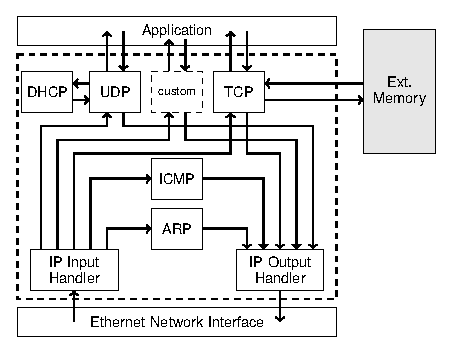
\includegraphics[scale=1]{introduction/fccm2015.eps}
\caption{The architecture of the Xilinx 10Gbps TCP/IP stack introduced in
\textit{Scalable 10Gbps TCP/IP Stack Architecture for Reconfigurable Hardware,
in FCCM’15}\cite{sidler2015tcp}.}
\label{fig:fccm2015}
\end{figure}



\chapter{Background}

In this chapter, we will introduce the basic concepts of the Internet Protocol
Suite, briefly describe its origin, semantics, and some of its protocols.
Furthermore, SME and the hardware it will run on will be introduced as a basis
for the implementation.


\section{Internet Protocol Suite (TCP/IP)}
Internet Protocol Suite, better known as simply TCP/IP, is a conceptual
model providing end-to-end communication between computers. It consists of
a collection of protocols specifying the communication between multiple
Internet systems\cite{RFC1122}.  The very early research and development
on what would later become the Internet Protocol Suite began in the late 1960s
by the Defense Advanced Research Project Agency (DARPA), and was being
adopted by DARPA, as well as the public, since 1983\cite{DARPA_internet}.
Although the Internet Protocol Suite predates the newer, arguably more
refined Open Systems Interconnection (OSI) model, TCP/IP still
remains the popular choice in modern systems.  As opposed to OSI 7-layer
model\cite{X.200}, the collection of protocols in TCP/IP are organized
into 4 abstraction layers, each related to their scope of networking
involved.

\subsection{Link Layer}
The link layer is the lowest, bottom-most layer in the Internet Protocol Suite.
Link layer addresses methods and protocols operating on the link that the host
is physically connected to\footnote{Wireless connections are also included
under this category.}. Contrary to the OSI model, this lowest layer in TCP/IP
does not regard the standards and protocols of the physical mediums used (the
pin layout, voltages, cable specifications etc.), making TCP/IP hardware-independent.
As a result, TCP/IP can in theory be implemented on virtually any hardware
configuration, emphasizing the flexibility of the model.

\subsection{Internet Layer}
The internet layer mainly concerns itself with sending data from the source
network to the destination network. This seemingly simple task requires multiple
functions from the layer:
\begin{itemize}
    \item Addressing and identification
    \item Packet routing
    \item \emph{Basic} transmit diagnostic information
    \item Carrying data for various upper layer protocols
\end{itemize}


\subsection{Transport Layer}
The transport layer establishes end-to-end data transfer between hosts.
Protocols in the transport layer can provide additional services to the user,
such as reliability, ordering, error- and flow-control, application addressing
(port numbers), error-checking, and so on.\\
While it is possible to bypass the protocols in this layer on most modern
network stacks, the protocols in the transport layer provide such essential
and useful services that it hardly ever makes sense to implement in the
application layer.\\
While there are numerous protocols defined in the Transport Layer, perhaps the
most well-known protocol in the stack is the Transmission Control Protocol (TCP).
Being one of the most used transport protocol for its reliability and congestion
control systems, it is rightly justified to refer to the whole Internet Protocol
Suite as simply "TCP/IP".


\subsection{Application Layer}
The application layer protocols are used by applications and services to
exchange information over the network. A few of the well-known application
layer protocols are the Hypertext Transfer Protocol (HTTP)\cite{RFC1945},
File Transfer Protocol (FTP)\cite{RFC0114}, and Simple Mail Transfer Protocol
(SMTP)\cite{RFC0788}.\\
This layer is usually implemented by the userspace applications themselves, and
therefore are not strictly required to actually run a TCP/IP network.



\section{Hardware}
The networking stack is intended to be flexible enough to run on just about any
configuration of hardware and software. However, this also means that it cannot
depend on any major external components, such as an existing memory, a processor,
or any form of operating system. Fundamentally, not only the software-part of the
networking stack has to be implemented, but the hardware needs to be defined
as well. This hardware should be self-contained enough to work well in combination
with any additional system, which the user incorporate for networking.\\
A wide variety of hardware types exist for such independent system, such as
Application-specific Integrated Circuit (ASIC), Complex Programmable Logic
Device (CPLD), Socket on a Chip (SoC), and Field-Programmable Gate Array (FPGA).
Each of these integrated circuits have their advantages and disadvantages; some
of them are re-programmable, some are cheap and disposable, and some are excellent
for general-purpose applications.\\
In this thesis, only FPGAs will be taken into consideration for its re-programmability,
its fairly low-cost, and the compatibility with SME code-generators.


\subsection{Field Programmable Gate Array (FPGA)}
Field Programmable Gate Arrays, or FPGA for short, are devices containing
integrated circuits (ICs) consisting of arrays of logic blocks.
These logic blocks can be programmed to form arbitrary logic circuit by simply
synthesizing a design and then loading it onto the board. This process alone
can save the manufacturer months by not having to fabricate a whole new IC. \\
FPGAs can be used for any computational tasks without the need of any additional
hardware. Usually, these devices are used for smaller, domain-specific tasks,
where the control over the hardware yields significant performance increases.
FPGAs are indeed very universal, and can be used in product-design, prototyping,
as well as in final products. Products like car driver assistance
systems\cite{xilinx_fpga_automotive}, audio decoders\cite{xilinx_fpga_audio},
or even internet search engines\cite{bing_search_fpga}  all utilize FPGAs to
increase the performance, lower the electrical bill, and  boost the development
potential.


\subsubsection{Technical specifications}
Field Programmable Gate Arrays consists of a vast number of ICs, which can
be reprogrammed at any time for a desired application or functionality\cite{ni_fpga},
making the devices very flexible and extensible, even after manufacturing.\\
These ICs are practically totally independent, and their logic within can be
programmed and combined in virtually any way with other ICs. This, however,
poses a problem, as signals do not propagate through circuitry, immediately, but
rather, they have a slight delay.
Sometimes, two events precede each other, while other times, events of distinct
timings must occur simultaneously.
Since the order of events is critical for correct and expected execution in
digital circuits, a digital clock is used to ensure everything runs in sync.
A clock in this context emits a series of pulses in a pre-determined and very
precise interval. These pulses are used to control the execution of various
elements in the circuitry.\\
When synthesizing to a FPGA, the compiler finds the longest code-path, it finds
the required circuitry to perform the calculation, and then it determines the
minimal required time for the signals to propagate through the path. In this
manner, the fastest possible clock can be found for that particular circuit.\footnote{
    Although many modern FPGAs consist of multiple regions which can have individual
    clock-rates. While it is a demanding task to propagate signals across these
    boundaries, a performance increases can be gained.
}
With innovations and steady improvements in modern FPGAs, the circuitries within
the devices can be clocked at higher than 500 MHz\cite{xilinx_fpga}.



\subsubsection{Programming an FPGA}
Unlike conventional processors with a very sequential nature, the logic blocks
in FPGAs are truly parallel in nature. Given the right programming, an FPGA can
allocate dedicated sections of the chip for each independent subtask, enabling
the circuitry to perform numerous independent calculations at once\cite{ni_fpga}.
Unfortunately, this universality of FPGAs comes at a cost to their performance.
Whereas conventional processors are heavily optimise based on the predetermined
circuitry, FPGAs programmers must ensure to utilize the parallel nature of the
device in order to secure best possible performance. Even worse, the FPGA must
be programmed in such a way that all paths in the electrical wiring can be
in any time-frame.\\
Due to this parallel nature of FPGAs, conventional programming languages are
next to impossible to use. To define the behavior of an FPGA, Hardware
Description Languages (HDL) are used. These programming languages are not easy
to learn without a good grasp of electrical engineering. Even with prior
programming knowledge, the unusual approach to concurrency in these languages
can be hard to understand for average developers.\\
To simplify the development process, most manufacturers offer predefined
circuits along their FPGAs. These predefined circuits are more commonly known
as Intellectual Property (IP) cores, and can provide the hardware designers
with pre-made circuitry for a wide variety of functionality. While most IPs
provide the functionality of processors for testing on an FPGA, mp3 audio
decoding or PCI bus interconnect can be obtained as well\cite{fpga_for_dummies}.



\section{Synchronous Message Exchange}
The Synchronous Message Exchange
model (SME) is a messaging framework created in order to help model
hardware descriptions\cite{sme_for_hardware_designs}.  It was conceived
once the flaws of using Communicating Sequential Processes (CSP) was
identified during the modelling of a vector processor with CSP using
PyCSP\cite{PyCSP}.  It turned out that there is a major discrepancy
between the way data is propagated in hardware opposed to that of the
CSP model. While CSP does not pose any requirements on the communication
between processes, in digital hardware, all communication has to be
synchronized, driven by a clock. To combat this in the CSP model, a
global clock process needed to be implemented, which was connected to
all other processes. Additionally, latches had to be introduced in order
to not overwrite values during a cycle. This caused an explosion of both
channels and latches in the final design, making CSP a much less viable
framework for hardware modelling\cite{sme_for_hardware_designs}.

\subsection{The model} The SME model consists of only a few fundamental
concepts. Each SME model is a \textit{network} consisting of one or more
\textit{processes}. These processes do not share any memory or storage,
but are interconnected with \textit{busses}.  These busses are perhaps
the most interesting units in SME model, as they not only propagate
information between processes using the underlying \textit{channels},
but also introduce an implicit clock between the processes.\\

\subsection{Process execution flow} The execution flow of a process is
fairly simple, and relates very closely to that of the actual hardware. At
the beginning of a clock-cycle, the input-ports are read into the busses
they are connected to. Then, the process executes its "compute" stage, and
the results, if any, are written to the output-port, which will be read
by the following bus. A visualization of the execution flow can be seen
on figure \ref{fig:sme_clock}.  \pic{0.5}{background/sme_clock}{An
illustration of a typical SME clock-cycle}{fig:sme_clock}
It is important to note that although certain channels might be written earlier
than others in a process clock, the subsequent processes connected to said bus
will first see the values change in the beginning of the next clock cycle.


\subsection{Using SME}
SME has undergone multiple iterations, reworks, and extensions. While
it is still under very active testing and development, its core
functionalities and features
 are well-established and stable\cite{bus_centric_sme}.\\
SME has concurrent implementations in the C\# and Python languages,
with promising efforts to unify these under a common intermediate
domain-specific language SMEIL\cite{smeil}. The C\# version has
exhibited various advantages over the Python counterpart, such as
the more error-prone strong typing system, which better reflects the
functionality of the hardware, as well as making the code more readable to
the programmer. At the time of writing, the C\# implementation currently
enjoys the most recent features of the SME model, as it is being the
most actively developed version.



\chapter{Design}
\label{chap:design}
% introduction about the network stack?

\section{Overview}
The networking stack introduced in this thesis is implemented in the C\#
programming language with SME. The aim of its design is to capacitate performance,
flexibility, and ease of use. In this chapter, the design principles are
described, the architecture of the solution is outlined, and the components are
outlined.


\subsection{Design principles}
As briefly mentioned in the introduction, the proposed network stack is to
provide an alternative to the existing proprietary network offloading engines.
While the main goal of this thesis is to research and study the suitability of
SME for implementing a TCP/IP stack on an FPGA, there are many other aspects of the
system to be studied.\\
The extensibility of the network stack are to be tested by studying the effects
of introducing new protocols to the stack. While the network stack should be
able to be refined with new and custom protocols, it is to be studied which
implications it has for the system. Mainly, it is to be seen how the addition
of new protocols affect the performance, scalability, and viability of the
system.\\
In the same vein, the design should be as FPGA-agnostic as possible. While this is
mainly guaranteed by the SME framework used to develop the system, the underlying
systems, operations, and features should be easily portable across FPGA manufacturers.\\
Lastly, the design of the networking stack should be interoperable with other
systems on the FPGA, or even FPGAs. It is to be seen how easy it us to modify
and extend the versatility of the system without any major modifications or
even extensible knowledge of the system. As an example, the networking stack
can be expanded with a firewall, developed alongside this project.

\subsection{Initial requirements}
Following our design principles, initial requirements and goals for the
networking stack are set so that these can be tested and improved upon.
\begin{itemize}
\item \textbf{Essential protocols only}\\
Considering that the SME project is still fairly early in its development, and considering
the sheer number of protocols in the internet protocol suite, the networking
stack in this thesis is to support only the absolutely essential protocols
required to provide the users with a meaningful interface to the internet.
These protocols should be picked such that the system can provide the end-user
with a network data-stream, which can transport information to and from a remote
computer.\\
The initial protocols chosen may be implemented and supported partially, but
they must not deviate from the standard specifications.

\item \textbf{Support an interface for the end-user}\\
The system must be controlled by an end-user on the FPGA. Such an interface is
very unique in its own way, compared to standard software interfaces, like the
ones defined in the POSIX collection of specifications. By supporting such an
external interface gains insight in the way such a networking stack will be used,
and which measures must be taken in order to provide the best possible integration
and performance considerations.

\item \textbf{Independent of underlying physical hardware}\\
By using SME, the underlying hardware description language code can be abstracted
away from the actual implementation. This will later provide developers to easily
modify and tweak the networking stack without having to consider the target
hardware.\\
Likewise, the networking stack may not rely on using a certain physical layer hardware,
and must be designed to be independent of the underlying hardware used for the
physical connections. This will ensure that the target hardware can easily
swap between physical connectors, such as going from ethernet cables to wireless,
or even another FPGA.
\end{itemize}

\section{Initial design}

% Spans 2 columns
\begin{figure*}
    \centering
    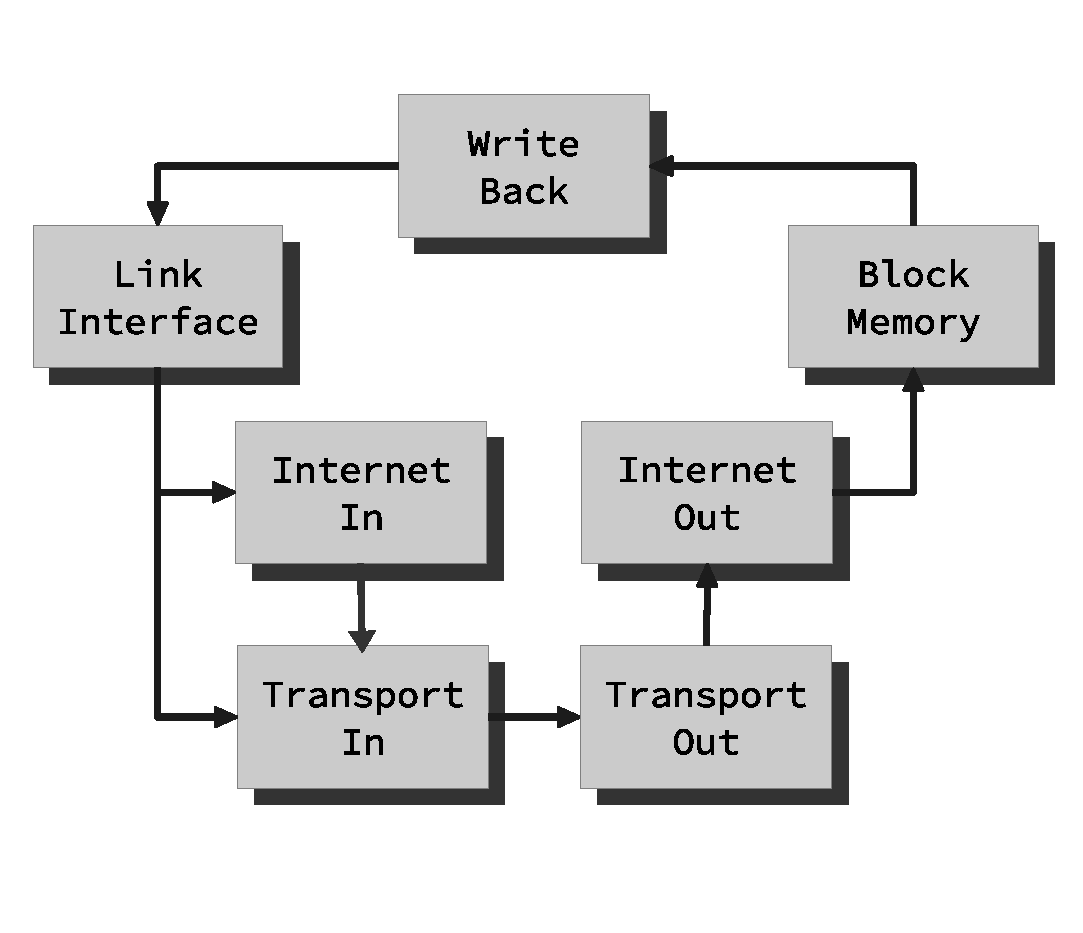
\includegraphics[scale=0.45]{design/design_0.eps}
    \caption{The initial design}
    \label{fig:initial_design}
\end{figure*}

The initial architecture had a very simplistic approach to its design in order
to aid with early identification of potential issues and problems.
The basic idea of the initial design is to minimize the number of memory
operations carried out. Under the assumption that the Ethernet interface used in the network
stack will likely have limited memory, everything needs to be copied directly to
the stack. Figure \ref{fig:initial_design} shows the initial design, where the
leftmost module Ethernet connects to the memory for direct access, and each
parsing layers listens to this connection and performs accordingly. Each parsing
layer also connects to the subsequent layer in order to flag when the subsequent
layer should start listening on the data-bus (that is, where the current packet
header stops and the next header begins).\\
An advantage that this design provided was the cetralized memory, which is much
easier to up-scale in terms of capacity and bandwidth. This global memory would
also be able to modify packets in-place, removing duplicate data, minimizing the
need to copy data around, and making it easier to keep track of the memory
fragmentation.

\subsection{The issues}
As anticipated, this initial design brought fourth the main issue fairly quickly
in the implementation phase, where most of these stem from the differences in
programming hardware as opposed to the software network stack, from which the
inspiration was drawn.

\subsubsection{Internal parsing buffer or memory is largely unavoidable}
Although listening to the global data-bus and processing on the bytes currently
therein  seems like an efficient way of minimizing the data-transfer required
across processes, it has shown to yield some unavoidable challenges.\\
Parsing fields in a packet-header is much more cross-dependent than initially
anticipated; each field might have numerious implications on the way preceeding
and subsequent fields are read and interpreted. As an example, in the Internet
Control Message Protocol (ICMP), a redirect message type has an IPv4 address field in
the header, whereas in the timestamp message type, this field is interpreted as
both an identifier and a sequence number.
This sort of inter-dependency is hard to parse without the ability of caching
or buffering the header locally in the parsing process.

\subsubsection{Overutilized memory module}
While the ethernet is the main writer to the memory module, the parsing layers
need to access and write to the module as well. At the very least, the memory
module would have 6 connections in the network, not counting any additional
components, such as user interface, firewall, etc.
Although numerous memory implementations exist on the FPGA landscape, Block RAM
(BRAM) seems to be the most suitable in this situation for its speed and latency.
Unfortunately, many widely used block RAMs only have 2 simultaneous connections
(or "ports") at the same time. Additionally, the block rams are frequently
limited to only operate a few bytes of data at a time.\\
Although some block RAMs, such as the ones found in Xilinx FPGAs can be cascaded\cite{xilinx_fpga_memory_resources}
to lessen the impact of these limitations, this hardly provides a good basis for
a scalable design.

\subsubsection{Data fragmentation and memory management}
Another problem a unified address space in the global memory is how costly
basic memory operations, such as moving or copying, become. The initial
assumption that packets stored in memory could be reused by modifying them
in-place and send them turned out to be misguided, since the layout, size, and
the number of the outgoing packets very rarely resemble the in-going packets.\\
Furthermore, the general purposeness of the memory makes it very hard to
structure. Without very complex memory management, the memory can get very
fragmented and slow.


\section{Revised design}
The initial architecture focused heavily on the input from the link interface,
minimizing hardware memory requirements, and to minimize the latency from the
source data-stream to its respective layer handler. Unfortunately, the opposite
revealed to be true, as the overly-utilized memory unveiled plentiful issues to
the performance.\\

\begin{figure}[h]
    \centering
    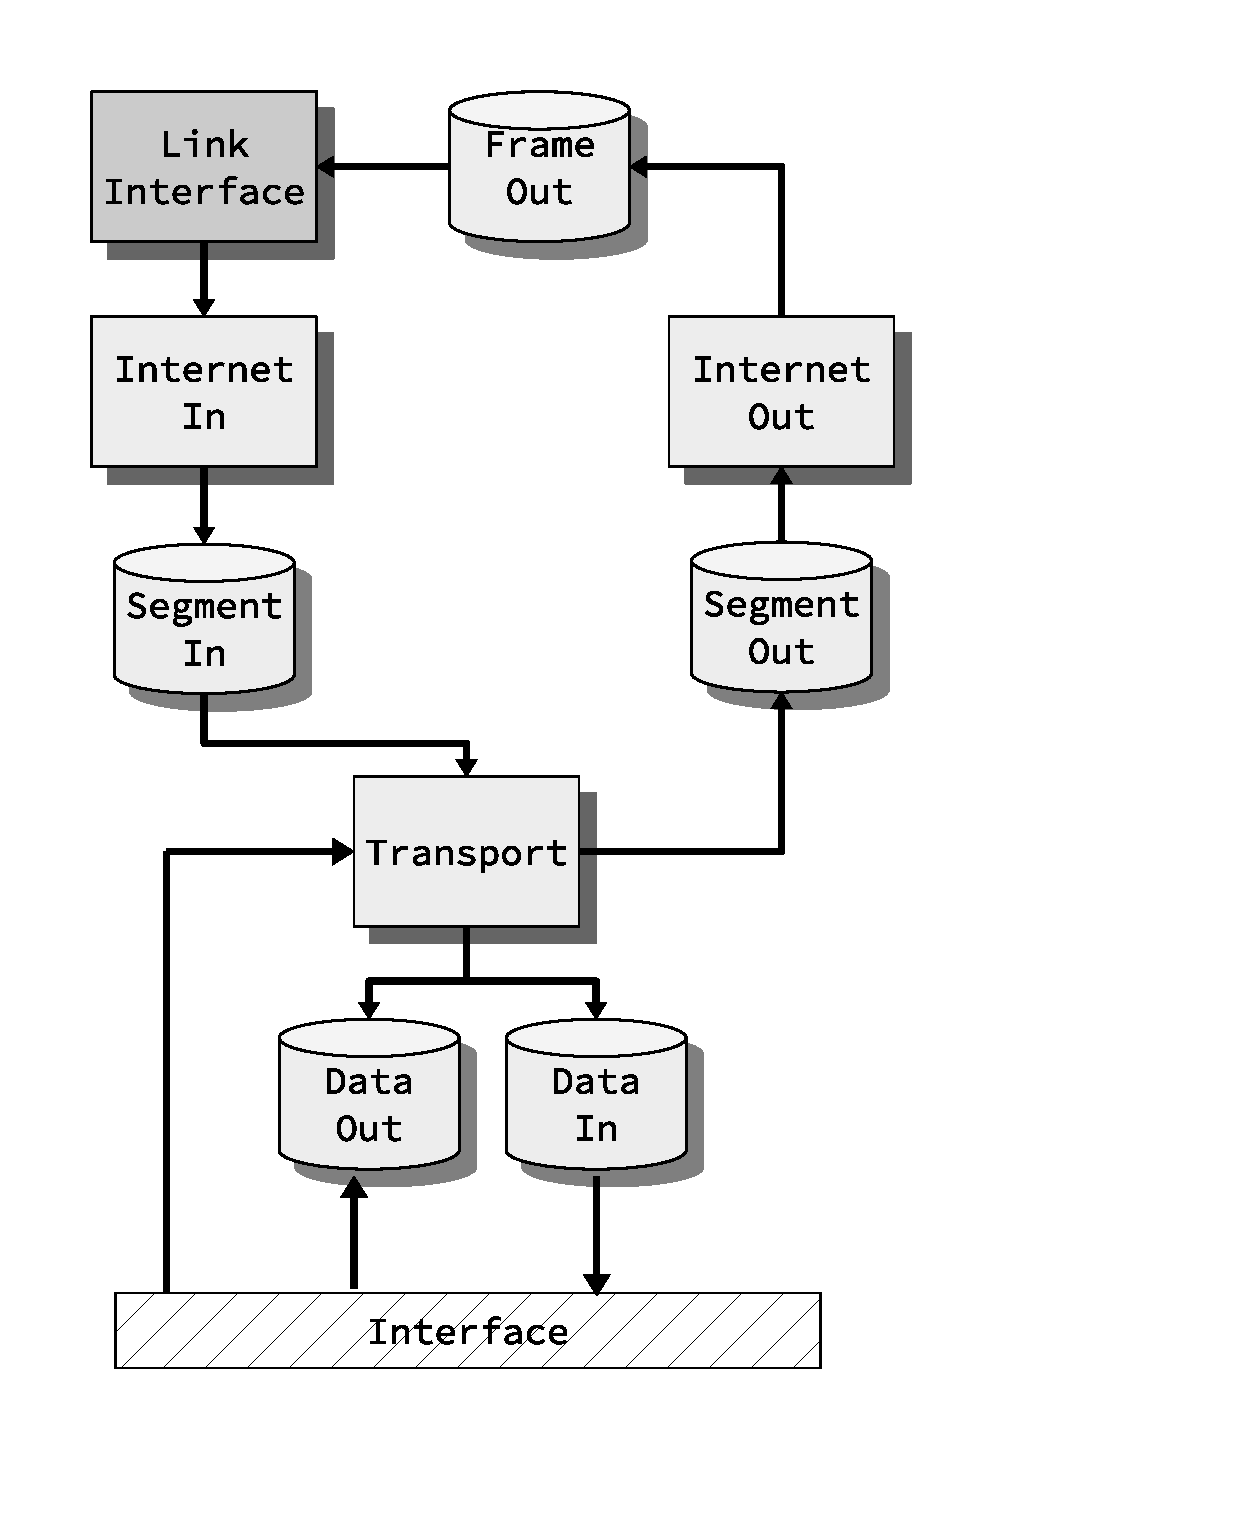
\includegraphics[scale=0.45]{design/design_1.eps}
    \caption{Second iteration of the design}
    \label{fig:second_design}
\end{figure}

To avoid the problem with global memory, the data needs to "flow" through the
components that need the data at that time. Therefore, as opposed to the initial
design, where the link interface writes to memory directly, in the revised design,
this connection is completely removed. The idea is to let all the data pass
pass through each state, letting each stage parse the required information, and
passing the rest to the next components.\\
As seen on figure \ref{fig:second_design}, the link interface, which
provides the raw byte-stream from the network, is connected to all of the input
parsing layers. The layers are connected in the order in which a network frame
is parsed; link- to internet- to transport-layer. This approach aims to utilize
the fact that the layers can act immediatelly upon the packets received directly
from the source, avoid having to buffer the whole packet in each stage, as well
as easing the logic required to buffer the data across the layers.\\
This design starts by the Link Interface sending one byte at a time through its bus.
The \texttt{Link In} will parse the first header, and signal the next layer upon completion.
\texttt{Internet In} will then start to listen on the \texttt{Link Interface} bus
and, using the information from \texttt{Link In}, parse the internet header
accordingly. The same procedure would be applied to the connection between
\texttt{Internet In} and \texttt{Transport In}.\\
When data is to be sent to the internet, the network frame would be built bottom
up from the transport layer through internet to the link layer.

\subsection{The issues}
The issues quickly surfaced during the implementation of this revised design. Although
the interconnect from the \texttt{Link Interface} to all the subsequent layers
in parallel promised negligible latency, it came with a great cost to the solution.

\subsubsection{Process under-utilization} \label{item:process_utilization}
Since each "in" process has to wait for the previous layer to signal when to
start listening on the data-bus, the layers would in average only be active a third
of the time. Since each layer has very little information about the states of
the other layers, it would become a challenge to get any other work done during
these phases.\\
For example, it would be an immense challenge to coordinate an ICMP reply on a
faulty packet in the \texttt{Internet In}.

\subsubsection{Redundant Link layer}
While the Link layer is an essential part of the Internet Protocol Suite, it did
not fit well with the functionality of the rest of the stack.
Most network interfaces are equipped with buffers, on which integrated circuits
perform operations such as error check using cyclic redundancy check, de-noising,
timeslot management, etc.
Likewise, the Pmod NIC100 Ethernet interface has built-in controller with
internal memory suited for buffering the incoming packets\cite{microchip_enc424j600}.
This memory, apart from the cyclic redundancy check, can be used as the initial
step for parsing the packet, and only send the datagram to the stack.


\subsubsection{IPv4 fragmentation and out of order TCP packets}
The chaotic nature of internet routing might cause packets to come out of order,
or even get fragmented along the way. Since each layer parses the packet immediatelly
as it is written to the bus, it became a challenge for the layers to figure out
what to do. On IPv4 fragmentation, if the second half of a dataframe arrived
first, the Transport header would not be available to the Transport layer.
Although IPv4 fragmentation is an increasingly rare phenomenon, the network
design is not able to handle the situation well.


\subsubsection{TCP connection state sharing}
With a clear separation between the "in" layers and the "out" layers, the
Transport block had to be split as well. Unfortunately, unlike the other stateless
layers, the transportl layer actually needs to keep track of the connections and
their states. On every segment received, the appropriate connection needs to be
updated accordingly.\\
In the TCP protocol, the connection state changes on both receiving and sending.
In this case, the \texttt{Transport In} and \texttt{Transport Out} have to
agree on a shared state. As these states can be quite large, and the should
support multiple connections at once, one large bus containing all the information
is not feasible. To solve this, a negotiation protocol may be introduced, however,
as pointed out in item \ref{item:process_utilization}, the processes are very
limited in their execution time. A negotiation would be very hard to achieve in
such circumstances.


\subsubsection{Problematic order of building and sending outgoing packets}
Outgoing packets are built in the reverse order of which they are parsed -- the
inner layers are built first, and then the packet grows outwards by adding new
layers on top of the existing one.\\
That in itself is not a problem, as the packet can be easily passed through the
network backwards from the last byte first. That is, the inner-layer of a packet
is passed on to the next layer first, then the header packet header is built,
and lastly, the header is passed on backwards.\\
However, this assumes that the next layer to process the packet is available at
all times in order to process the packet. This is certainly not the case, as
layers such as \texttt{Link Out} and \texttt{Internet Out} might be in the
process of sending out their own protocol-specific control messages (such as
an ARP annoucement in the Link Layer or ICMP reply in the Internet Layer).\\
A negotiation protocol can be implemented between the outgoing processes in to
postpone the outgoing packet, but these structural hazards, as known from
conventional processor pipelines, add a lot of complexity to the system.





% \subsubsection{Control and logic flow}
% Although the layers take turns to parse the incoming byte-stream, the design
% handles the whole packets at once. This leaves

\section{Pipelined design}
While it would be possible to work around these identified issues with the
revised design in the code, the
added complexity would have additional ramifications on the project as a whole.
Upon further analysis of analysis, it is clear that the source of the issues is
the parallel arrangement of the process blocks.

\begin{figure}
    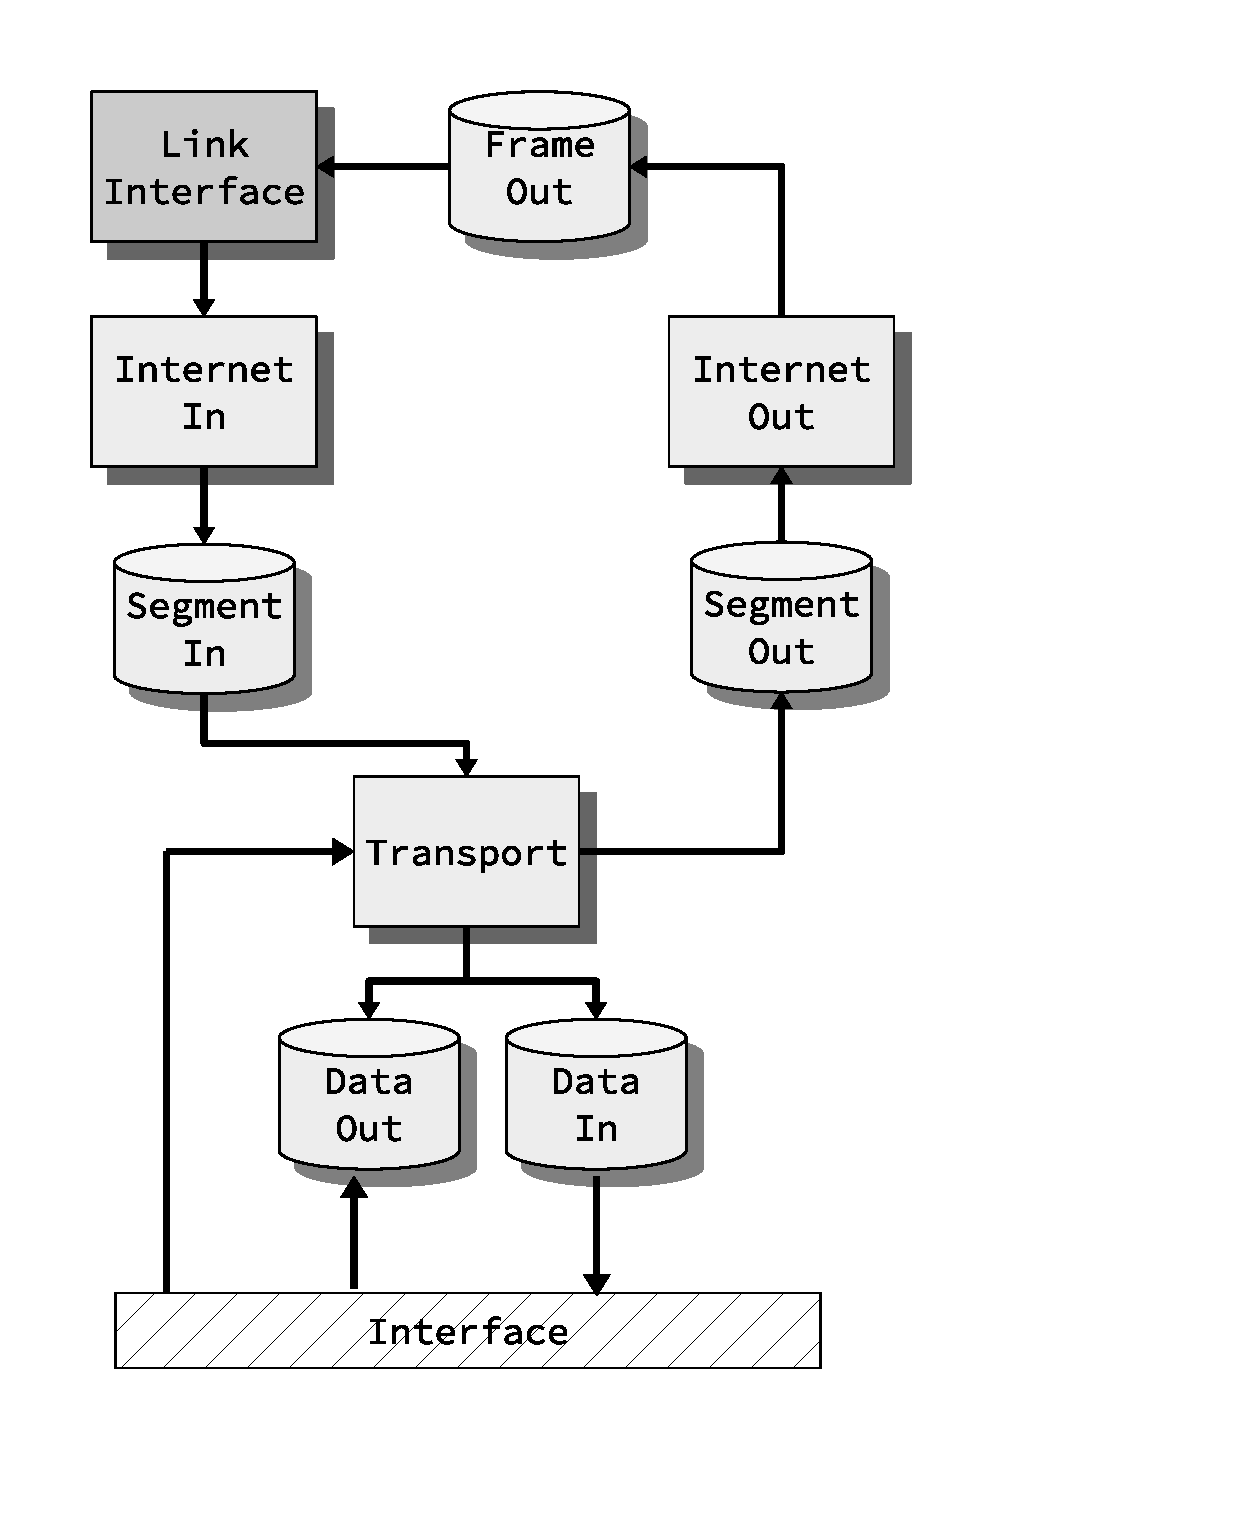
\includegraphics[scale=0.45]{design/design_2.eps}
    \caption{The final design. The rectangles represent "compute" processes,
while the cylinders represent the buffers.}
    \label{fig:final_design}
\end{figure}

The next iteration of the design utilizes a fairly standard approach to
pipelining, albeit with an unusual transfer of data between the stages.\\
The idea with the pipeline is to enable the processes to receive, compute, and
forward data at their own pace, without any major limitation from the other
parts of the system.

\subsection{Internet layer processes} \label{sec:layer_processes}
The processes performing computation and processing on the actual internet
packets, called "layer processes" for brevity, are by large kept intact from the
previous design. The fairly simple, but highly sequential nature of packet
header parsing turned out to be very complicated to optimise with the additional
computing power of the hardware, without introducing too much complication.\\
Missing from the updated figure \ref{fig:final_design} are the \texttt{Link In}
and \texttt{Link Out} processes, which, for now, are handled by the ethernet
interface, which can easily parse and strip the first frame headers.


\subsection{Busses}
The busses in the revised pipelined design are devised such that communication
is only limited to the immediate neighbours in the logical network. This design
is put in place so that the synchronization and the order of execution is much
easier to keep track of, so that fewer race-conditions occur, and so that blocks
in the network are easier to replace, remove, or modify, without having a large
cascade effect on the whole network, as opposed to only the neighbours.\\
Whereas in the previous design where the busses would simply write new data on
every new clock-cycles regardless of the reading processes, now there must be
some logic to actually ensure that the reading process is ready to receive new
data. While the Data Buffers, as introduced in the next section \ref{sec:data_buffers},
solve the issue of blocks reading and writing data at their own pace, the busses
must support an interface for sharing the state of both processes. Thus, while
the busses are depicted as directional with arrows in figure \ref{fig:final_design},
there is naturally a need for a control signal in the opposite direction to
control the data-flow. This communication protocol will be discussed further in
the implementation section \ref{sec:interface_signal_protocol}.


\subsection{Data buffers} \label{sec:data_buffers}
Illustrated as cylinders on figure \ref{fig:final_design}, First-In, First-Out (FIFO)
buffers are introduced between each parsing process in order to control the data-flow
between the layers. Apart from maintaining a fairly large memory bank through
the block-RAM, these buffers also contain logic to store the incoming data
intelligently in order to offload the following processes. For example, the
\texttt{Segment In} buffer ensures that fragmented IPv4 packets are defragmented
before leaving the buffer.
However, introducing a new "type" of a process --- the buffers --- poses a new
challenge. While the buffers can be read from at any time, the layer-parsing
processes do not have this luxury, as they do not have any significant internal
buffer. Here again it becomes obvious that a handshake protocol needs to be used
in the bus-communication between the buffers and the processes.

\subsubsection{Order of outgoing packets}
In the previous design, it was obvious how sending packets might become a challenge
given that all processes involved must be ready to promptly operate on the
outgoing packet. With the introduction of data buffers, the processing of an
outgoing packet can be delayed.
However, there lies another small problem with the way data is passed around.
The \texttt{data}-section has to be read by Transport in first-in, first-out
order, solely for the reason that Transport does not know beforehand how much
data to send, nor whether more urgent tasks appear during the transmission.
Figure \ref{fig:sending_packet_order} shows the possible ways of creating and
passing a packet along the network stack.
\begin{figure}
    \centering
    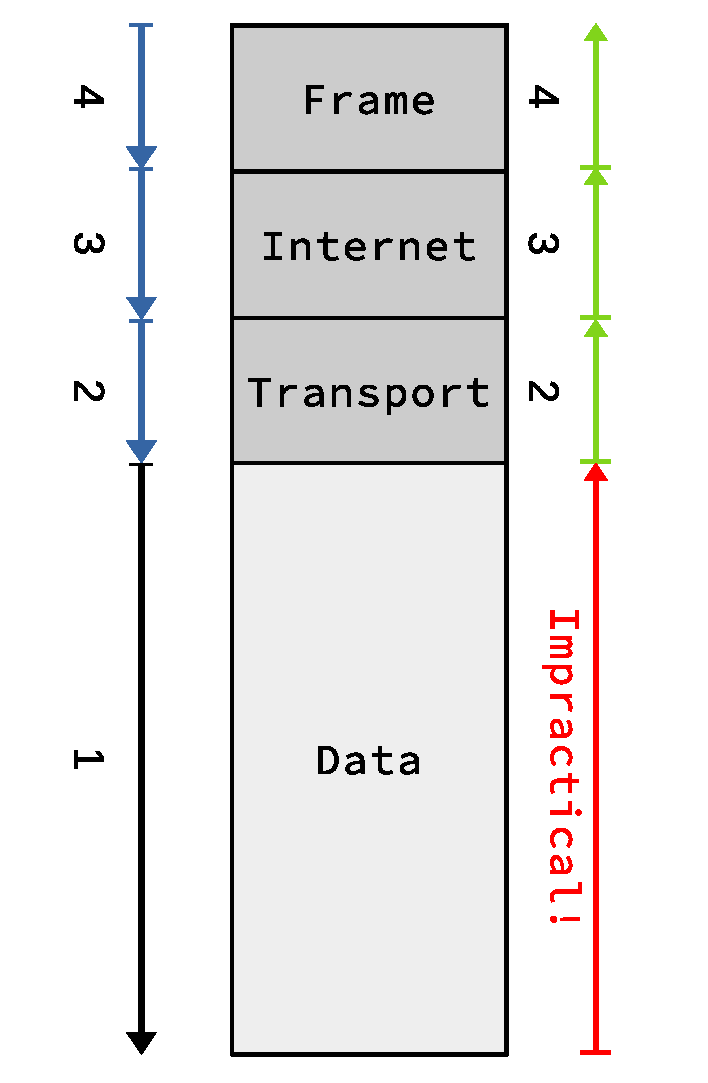
\includegraphics[scale=0.45]{design/sending_packet_order.eps}
    \caption{Possible orders of ways of building an outgoing packet}
    \label{fig:sending_packet_order}
\end{figure}
On the right side of figure \ref{fig:sending_packet_order}, the data is sent
from the last byte first, indicated by the red arrow from bottom up. Then, the
transport-, internet-, and lastly, the frame-header is built and sent with it
in the same order, from the last byte of the header till the first.
While this method is fairly simple, it has two problems that are hard to work
around -- firstly, the user might be in the process of writing outgoing bytes
to the \texttt{Data Out} buffer, in which case, Transport cannot beforehand
start sending the last byte. The second problem is that, although Transport
wants to send as much data at once as possible to lessen the overhead from the
rest of the package, more urgent tasks might come up during the transmission,
yet the operation has to finish reading the last (first) byte.\\
The left side of figure \ref{fig:sending_packet_order} shows another approach
to sending a packet. Here, the data portion of the packet is read as is in the
first-in, first-out byte order. The headers are written afterwards, also in the
FIFO order. It is important to notice that even though the package looks
structurally right when reading backwards (the frame header is in the beginning,
then Internet header and so on), the ordering of the bytes is not correct! For
example, if reading the right-hand on figure \ref{fig:sending_packet_order}
packet in reverse order, the data section would begin with the very last byte!\\
Here, the intermediate buffers once again offload this problem, as one of the
brilliant features is that they enable the system to pass bytes out of order.
In that case, the sending process can begin in the middle of a package, and then
append to the beginning of it at the very last.\\
Figure \ref{fig:sending_packet_graph} shows the building of an outgoing packet.
Between each process, the colored block represents the state of the packet
being passed along the processes. The red arrow indicated the first stage of
the connection between processes, where data is passed from a previous layer.
The blue line indicates the data that the process itself appends to the stream.\\
The implementation of this out-of-order forwarding will be described in-depth
in the implementation chapter \ref{chap:implementation}.

\begin{figure*}
    \centering
    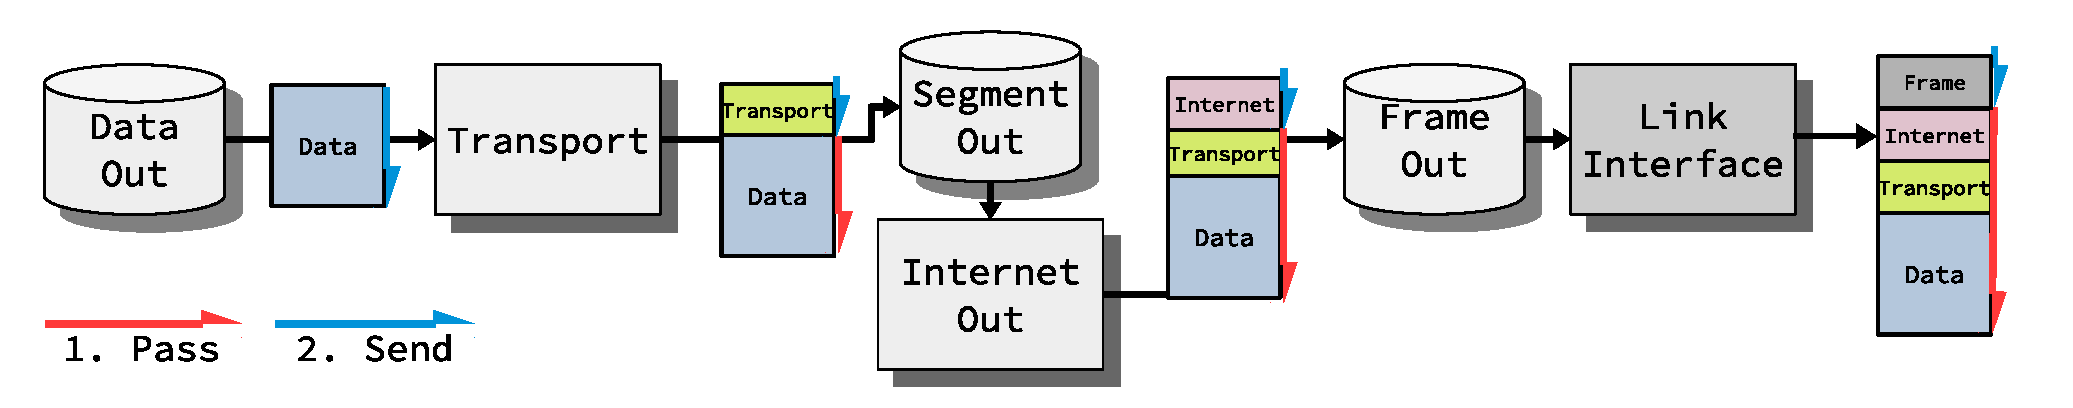
\includegraphics[scale=0.45]{design/sending_packet_graph.eps}
    \caption{The order in which an outgoing packet is built and passed through the network pipeline.
    The colored boxes represent the state of the outgoing packet, the red arrow
    indicates the first stage of forwarding, and the blue line indicates the last stage.}
    \label{fig:sending_packet_graph}
\end{figure*}



\subsection{Interface}
Lastly, the Interface is designed so that the end users and system can utilize
and use the network stack.\\
The networking stack is controlled with 3 connections (consisting of bus-pairs):
the control-, the read-, and the write-connection. While the last two connections
are incredible simple and only transfer data from the \texttt{Data} buffers,
the last connection controls the whole network-stack.

\subsubsection{Read/Write interface}
In conventional programming languages, the user would usually supply the a
function call with an array or a list on which the function can operate.
However, in hardware, this is generally not the case, as arrays are costly to
transmit at once.\\
Therefore, the two read and write interfaces would simply stream one byte at a
time, and it is up to the user to be prepared to read or write the data.


\subsubsection{Interface Control Bus}
The Interface Control Bus controls all the "business" logic of the network --
maintaining the active connections, starting and closing connections, and various
other protocol-specific control on each connection.\\
Currently, all this can be handled by the \texttt{Transport} block which has all
the necessary information to handle the interface requests.\\
The design of the Interface is based on the widely adopted Berkeley Sockets library,
which saw the first implementation in 4.2BSD, and has been defacto a standard
component in the POSIX specification\cite{tcpip_illustrated_vol2}. There are
multiple reasons for this decision:
\begin{itemize}
\item The Interface will feel more familiar to users accustomed to the Berkely
Sockets API commonly found in mainstream systems such as Linux, OSX, and BSD
variants.

\item The inner workings of the stack will be more transparent, and the API
exposes fairly fine-tuned control over the whole network stack.

\item Even with the relatively few functions exposed, the API
has thrived in the most used systems as of now. It would be an understatement to
say that the Berkeley Sockets API have stood the test of time, and therefore, it
is a good basis for the interface used in the network stack.

\end{itemize}

The first version of the stack should support the following functions:
\begin{description}
\item[\texttt{listen(protocol, port)}]\hfill\\
    Finds and initializes a free socket with the given protocol and port. This
    socket is immediatelly put into listen mode.
    Returns error if protocol is not supported, if port taken, or if no free sockets
    are available.
\item[\texttt{connect(protocol, ip, r\_port , l\_port])}]\hfill\\
    Connects to a remote endpoint on \texttt{ip:remote\_port} using \texttt{protocol}.
    This call is used mainly by connection-based protocols that need to
    establish a connection before exchangning data, although it can also be used
    by datagram-based protocols as a way of setting the default destination to
    send subsequent data to.
    Returns error if protocol is not supported, if no free sockets are available,
    or if the optional local port is taken.

\item[\texttt{accept(socket)}]\hfill\\
    Accepts the pending connection and sets up the underlying socket state
    accordingly. Note that unlike the POSIX implementation of \texttt{accept},
    which returns a new socket with the connection, this implementation changes
    the state of the current, listening, socket.
    Returns error if no pending connection to accept, or if invalid socket
    supplied.

\item[\texttt{send(socket, byte, [ip], [port])}]\hfill\\
    Queues a byte for sending through the socket. An optional IP address and
    port can be specified in certain connectionless protocols.
    Guaranteed to succeed, given that the transport-bus can be written to. More
    on this discussed later.
\item[\texttt{recv(socket)}]\hfill\\
    Reads (or "receives") a single byte from the socket. The appropriate error
    code is set if no byte available on that particular socket.

\item[\texttt{close(socket)}]\hfill\\
    Closes the connection on \texttt{socket} and frees the socket for further
    usage. Calling on an already closed on non-existent socket has no effect.
    Guaranteed to succeed.

\end{description}

While the arguably most essential functions have been defined, there are some
functions from the Berkeley Sockets API that have been omitted for purely
technical and practical reasons.\\
The function \texttt{socket()} is mainly used to allocate and create new sockets
in an environment, but given that the hardware network stack has static allocation
of the sockets, it is not needed.\\
Additionaly, the \texttt{bind()} function is also missing for the sole reason
that in the current implementation of the network stack does not have any valid
reason not to bind a socket immediatelly.


% \cofeAm{0.7}{0.75}{2}{80}{0}


\chapter{Implementation}
\label{chap:implementation}
In this chapter, the implementation of the network stack using the
pipelined design from \autoref{chap:design} is outlined and described,
the application of SME detailed and evaluated, and lastly, the viability
of the system on an FPGA is discussed.\\

The network stack is implemented in C\# using the C\# version of SME, which is,
at the moment of writing, more mature and feature-rich. The current version of
the implementation supports most of the absolutely vital parts of the IPv4
protocol, as well as the UDP protocol, as specified by RFC 1122\cite{RFC1122}.
Although work has been carried out in order to ensure that additional protocols
can be implemented without obstructions, no additional protocols are supported
at the moment.\\
The solution is fairly well-divided into 3 different types of components,
relating closely to those of SME: processes, buffers, and busses. The most
interesting parts of these components will be described in further detail in the
following sections.


\section{Processes}
The processes are arguably the most vital part of the system, as they provide
the computation and "processing" on the in- and out-going packets.
It is important to note that although there are many other types of "processes",
in the network, such as the buffers, we will mainly refer to the modules doing
actual business-logic as "processes" \notelookup{Did we?} \footnote{These processes are not to be
confused with SME processes, which are used for the implementation of both the
buffers and processes.}.

The essential processes in the network are represented as light-grey boxes in
the \autoref{fig:final_design}. These processes are \texttt{Internet\_In},
\texttt{Internet\_Out}, and \texttt{Transport}.


\subsection{State-machines}
Network communication consists of countless different packets, formats,
protocols, combinations of flags and settings, and even errors and corrupted
bits. The processes in the network have to take on a manifold of jobs in order
to handle all these scenarios, which sadly cannot be handled with a simple
combinational logic circuit. To operate under these various conditions, these
processes are modelled as finite state machines, maintaining a single state at
all times.\\
The processes have a lot of similar states, such as \texttt{Idle}, \texttt{Receive},
\texttt{Pass}, or \texttt{Send}, but these can work very differently, as shown
in the following sections. Before moving on to describing the state-machines of
the 3 processes, it is crucial to understand how these can be modelled in SME.

\subsubsection{SME process execution flow}
To implement a process in SME, the C\# class has to inherit from
either the \texttt{StateProcess} abstract class, or the more simple
\texttt{SimpleProcess} class.
The latter class is, as its name states, a simpler version of the former. This
class implements an \texttt{OnTick()} method, which is invoked once for every
clock-cycle.\\
The more advanced, but also more capable \texttt{StateProcess}
class provides an abstract method \texttt{Run} which is to be overriden and filled
with the code desired to be run in the process. The interesting feature
about this method is that it is asynchronous, meaning that the code can
execute other tasks while waiting for resources, such as functions,
to return. In this case, this asynchronous feature is used to give
the programmer ability to split the function into multiple segments,
separated by the clock signal.\\
\autoref{fig:example_fsm} compares these two approaches for the same
finite state-machine with 3 consequtive states.

The "synchronous" approach using a \texttt{SimpleProcess} in subfigure
\ref{fig:sme_example_process_sync_code}
\notemark{Fix autoref}
has to implement a
variable tracking the current state of the process. On each new clock, this
state has to be analysed and the inteded function to be called based on the
value. This approach requires a lot of approach and boilerplate code, especialy
if there are several states.\\
The asynchronous approach on subfigure
\ref{fig:sme_example_process_async_code}
\notemark{Fix autoref}
on the other hand can do with only
single \texttt{Run()} method split into three parts -- A, B, and C.
After each code-segment, the process waits for the clock signal, and
continues with the execution of the next segment.  This functionality
gives the programmer a very granular control of the way a process
works, how it is split into multiple steps on the hardware, while
maintaining simplicity, as seen on the statemachine diagram on subfigure
\ref{fig:sme_example_process_fsm}.
\notemark{Fix autoref}

\begin{figure*}
    \begin{subfigure}[b]{0.3\textwidth}
        \centering
%\begin{lstlisting}[language={[Sharp]C}]
\begin{mintedcsharp}
public class SomeProcess : StateProcess
{
  private override async Task OnTickAsync()
  {
    // A
    await ClockAsync();
    // B
    await ClockAsync();
    // C
    await ClockAsync();
  }
}
\end{mintedcsharp}
%\end{lstlisting}
        \caption{Example using inheriting from \texttt{Process}, using the \texttt{Run()} asynchronous method.}
	\label{fig:sme_example_process_async_code}
    \end{subfigure}
\hfill
    \begin{subfigure}[b]{0.3\textwidth}
%\begin{lstlisting}[language={[Sharp]C}]
\begin{mintedcsharp}
public class SomeProcess : SimpleProcess
{
// Initial state
state = A;

protected override void OnTick()
{
  switch(state) {
    case A:
      a();
      state = B;
    case B:
      b();
      state = C;
    case C:
      c();
      state = A;
  }
}
\end{mintedcsharp}
%\end{lstlisting}
	\caption{Example pseudocode of using a "synchronous" \texttt{SimpleProcess}.}
	\label{fig:sme_example_process_sync_code}
    \end{subfigure}
\hfill
 \begin{subfigure}[b]{0.3\textwidth}
        \centering
        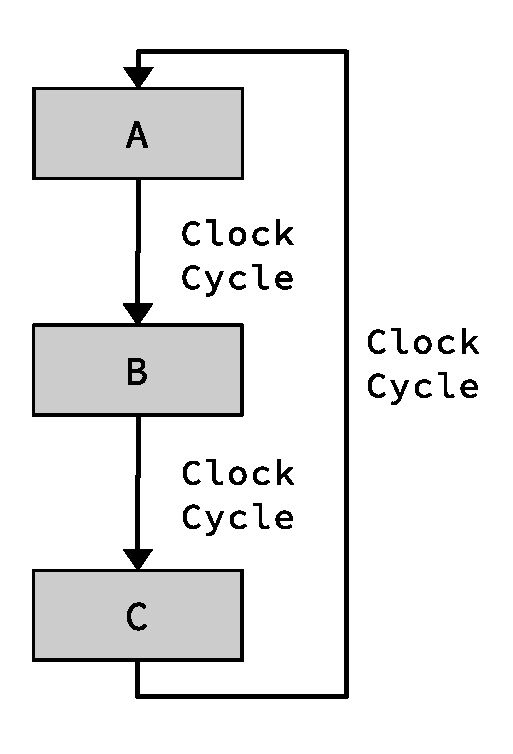
\includegraphics[scale=0.45]{implementation/empty_process_fsm.eps}
        \caption{The statemachine resulting from both code-examples. \\}
 	\label{fig:sme_example_process_fsm}
\end{subfigure}
    \caption{A simple state-machine implemented in the asynchronous (left) and
synchronous (right) approach in SME using C\#}
    \label{fig:example_fsm}
\end{figure*}


\subsubsection{\texttt{Internet Out} state machine}
This way of modelling a process in SME first the \texttt{Internet Out} process
very well, as it only has one responsibility, which is reading outgoing segments
and wrapping them in an Internet header. The \autoref{fig:internet_out_implementation} shows the pseudo-code and state-machine for the \texttt{Internet Out}
process. This process was easy to model and implement, because it only has one
input and one output, and the state-changes are simple and intuitive.

\begin{figure*}[htpb]
    \centering
    \begin{subfigure}[b]{0.45\textwidth}
        \centering
%\begin{lstlisting}[language={[Sharp]C}]
\begin{mintedcsharp}
public partial class InternetOut: StateProcess
{
public override async Task OnTickAsync()
{
  while segment_available() {
    pass_segment();
    await ClockAsync();
  }

  while header_available() {
    send_header();
    await ClockAsync();
  }
}
}
\end{mintedcsharp}
%\end{lstlisting}
        \caption{Pseudo-code for the \texttt{InternetOut} process.\\}
	\label{fig:internet_out_pseudocode}
    \end{subfigure}%
    \hfill
    \begin{subfigure}[b]{0.45\textwidth}
        \centering
        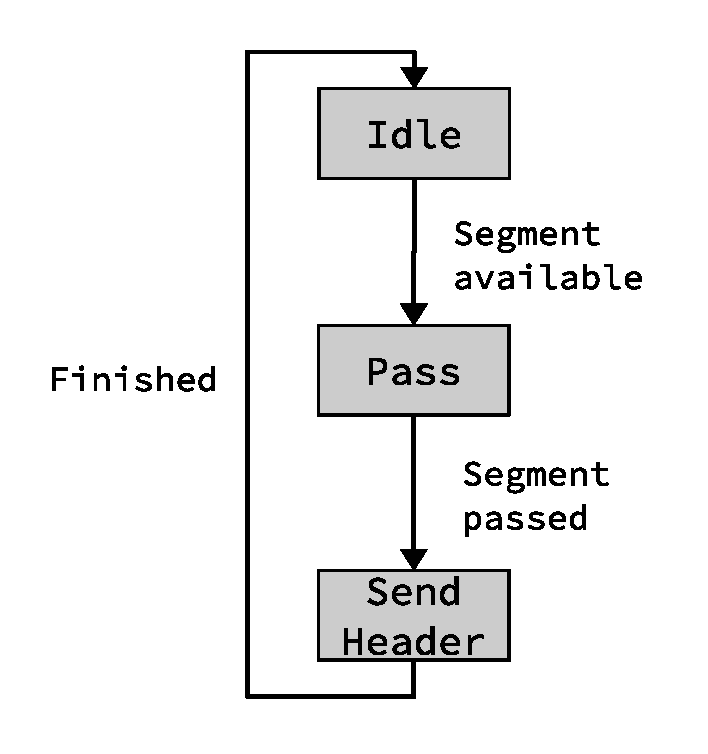
\includegraphics[scale=0.45]{implementation/internet_out_fsm.eps}
        \caption{The statemachine for the \texttt{InternetOut} process}
 	\label{fig:internet_out_fsm}
    \end{subfigure}%
    \caption{The implementation of the \texttt{InternetOut} process.}
    \label{fig:internet_out_implementation}
\end{figure*}


\subsubsection{\texttt{Internet In} and \texttt{Transport} state machines}
Unfortunately,
The state-machine of \texttt{Internet In} is probably the most simple of all the
state-machines, as it can effectively only read new packets from the Link-layer,
and pass it along the pipeline. Although it might be desireable for the Internet
layer to send control packets out to the network, this is not supported in the
current build.\noteinfo{Mere angående transport state machine?}



\begin{figure*}[t]
    \centering
    \begin{subfigure}[t]{0.5\textwidth}
        \centering
        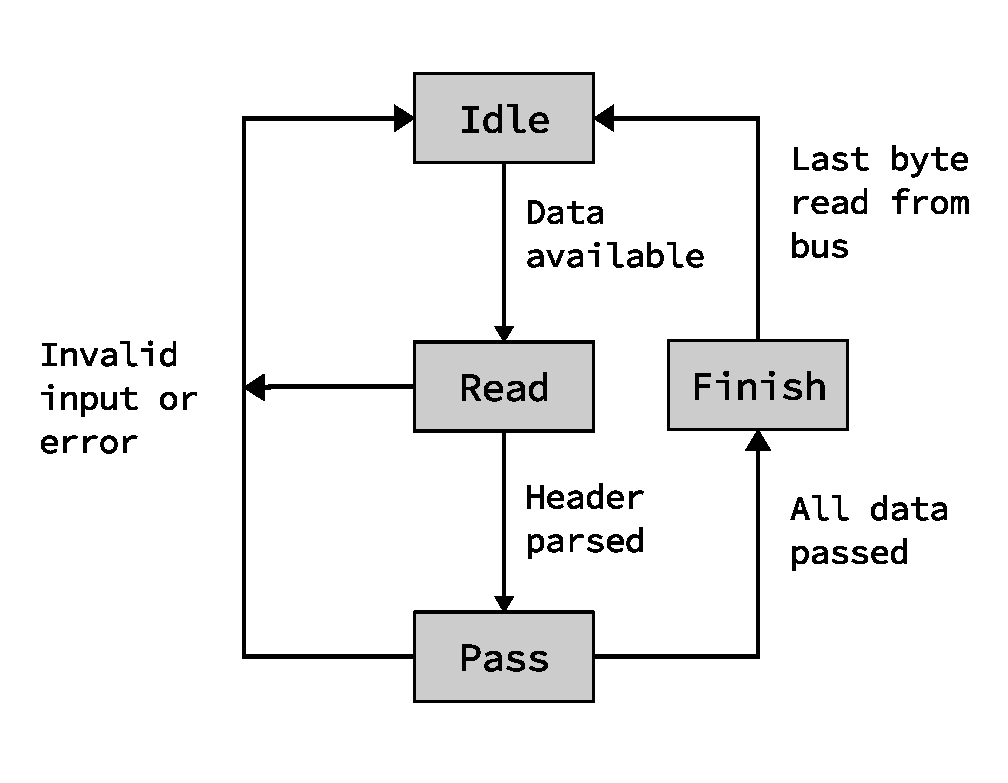
\includegraphics[scale=0.45]{implementation/internet_in_fsm.eps}
        \caption{The \texttt{Internet In} state machine}
    \end{subfigure}%
    \begin{subfigure}[t]{0.5\textwidth}
        \centering
        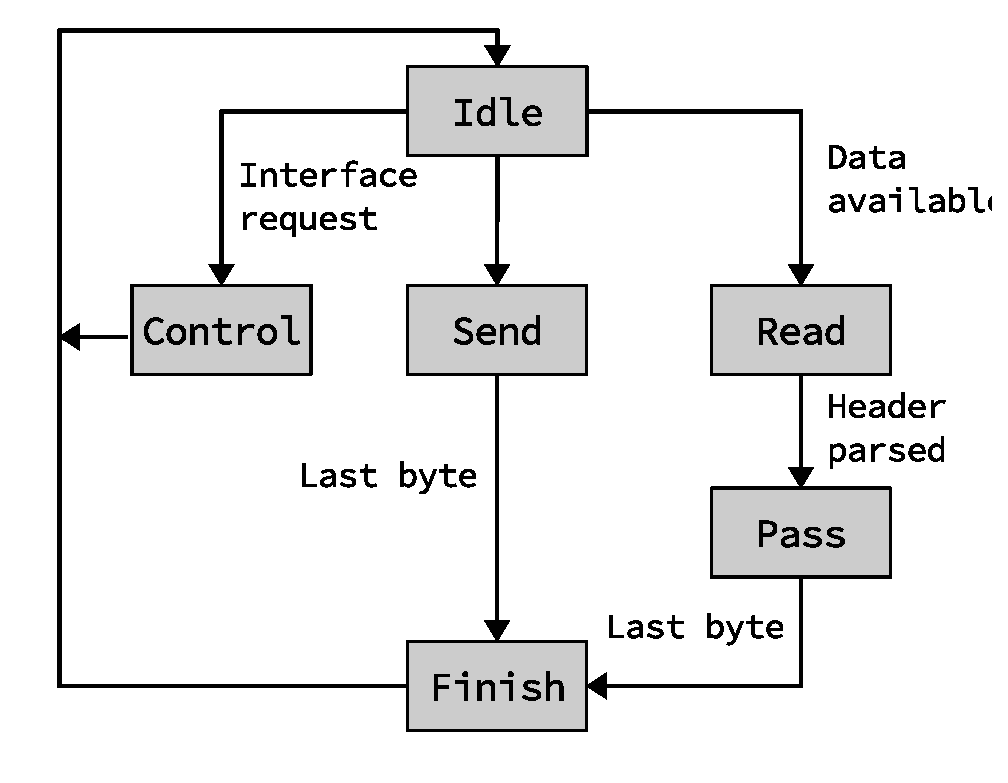
\includegraphics[scale=0.45]{implementation/transport_fsm.eps}
        \caption{The \texttt{Transport} state machine}
    \end{subfigure}%

    \caption{Statemachines for \texttt{Internet In} and \texttt{Transport}}
    \label{fig:statemachines_internetin_transport}
\end{figure*}


\section{Buffers}
Problems such as packet fragmentation and out of order insertion are solved in
the memory buffers.\\
All of the buffers needs to handle input and output of
memory at the same time. If not, the system would slow down by a factor of two,
since the input would need to wait for the output to finish submitting, and
vice versa. This requires the underlying memory to handle read and write in
parallel. \\
Each of the memory buffers have slightly different variations because
there are different problems to solve in all of them. In general, the problems
are the following: \notemark{Mention latency stuff}

\begin{itemize}
    \item \textbf{Fragmentation/Segmentation}\\
    In \texttt{Segment In} and \texttt{Data In} there are segmentation. In
    \texttt{Segment In} IP fragments may arrive out of order, and is therefore only
    sent through the system when all segments are received. \texttt{Data In} is
    essentially the same, just with other protocols such as TCP.\\
    In both cases we want the order to be concurrent. Packets that are not
    segmented is in FIFO order. Segmented packets in \texttt{Segment In} are
    held back, until all segments are received. Then all data segments are sent
    as a single block to \texttt{Transport}. In \texttt{Data In}, the segments are
    handled as a stream, where the last valid segment ID is known. The buffer
    only sends data when the last valid segment is updated. This way, the buffer
    can contain segments with an higher ID than the valid, and only send the ones
    that are smaller than the currently valid ID.


    \item \textbf{Unknown size}\\
    Some of the buffers do not get information about how much data has to be
    allocated. This happens in \texttt{Segment Out} and \texttt{Data Out}.
    In \texttt{Data Out} we do not know how much data the user sends into
    the system. (see: \autoref{subsubsec:interface_control}). In
    \texttt{Segment Out} we do not know some of the packet sizes, since
    \texttt{Transport} may not know beforehand how large the packet is going to
    be.

    \item \textbf{Out-of-order submission}\\
    In Some cases the header of an packet can only be created after the data
    has been received. An example of this is the calculation of the checksum.\\
    This feature is required on \texttt{Frame In} and \texttt{Frame Out}.
    This only applies to buffers where data is sent out of the network stack.

    \item \textbf{Data ready}\\
    When the buffer indicates that data is ready to be read, the next clock
    should also be ready and contain data. If not, the consumer would request
    data, wait at least 2 clocks for the data, and then request new data,
    slowing down the data transfer process significantly.

\end{itemize}
An oversight of this can be seen in \autoref{tab:buffer_requirements}.\\
\begin{table}[htpb]
  \begin{center}
      \begin{tabular}{l|c|c|c|c|}
          & \tablerot{Fragmentation}
          & \tablerot{\makecell{Unknown size}}
          & \tablerot{\makecell{Out-of-order \\ submission}}
          & \tablerot{\makecell{Data ready}} \\\hline
          \texttt{Frame Out}   &            &             & \checkmark & \checkmark \\ \hline
          \texttt{Segment In}  & \checkmark &             &            & \checkmark \\ \hline
          \texttt{Segment Out} &            & \checkmark  & \checkmark & \checkmark \\ \hline
          \texttt{Data In}     & \checkmark &             &            & \checkmark \\ \hline
          \texttt{Data Out}    &            & \checkmark  &            & \checkmark \\ \hline
      \end{tabular}
  \end{center}
  \caption{The requirements for the buffers} \label{tab:buffer_requirements}
\end{table}
\subsection{Components}
This section describes the components briefly to give a better overview of the
general structures of the buffers. The specific components are described in
detail in the following chapters.\\
To solve fragmentation the system uses "segments" in the memory.
A segment is an abstract structure consisting of metadata and two memory
addresses pointing to the start and end of the actual data.\\
To handle these segments, two interfaces are created, one to handle fixed size
allocations, and one to handle dynamic allocations, where the size is unknown.
Out-of-order submissions are solved simply by having an address sent beside the
data, which are added to the beginning of that respective segment.
See \autoref{subsec:memory_segments} for a in depth explanation.
\\
To keep order of the segments, a simple directory of keys and lists
are needed. The list are ordered at insertion time, so the fist element
always is the smallest. This makes lookup to the next element constant time, and
insertions of new at most $O(n)$ time. See \autoref{subsec:dictionary}.
\\
To have the data ready, a small internal buffer is needed. This small buffer
starts filling as soon as a segment is ready.
See \autoref{subsec:memory_types}.

\subsection{Memory segments} \label{subsec:memory_segments}
The memory segment structures consists of two types with slightly different
implementations. These are called Multi memory segments and Single memory
segments.
\\Their differences are explained at the end of this section.\\
Both types consists of an lookup table, where each table entry contains
metadata, head and tail pointers. A Illustration of this can be seen in
\autoref{fig:memory_segments_explained}\\
In the implementation, the memory is not actually read, but an address is
returned. This makes it possible to use any memory type, since the latency issues
are in the submission and retrieval of the data itself, but not the calculations
for the address.\\
The lookup table consist of multiple segments references. A segment reference
contains meta data(Not illustrated in the figure) and a start and stop pointer.\\
In the illustration segments 0,1 and 4 are used, and 2 and 3 are free. Note that
segment 4 wraps around. If address 2 is requested from segment 4, memory address
15 is returned. If address 3 is requested, memory address 0 is returned.\\
\begin{figure}
	\centering
	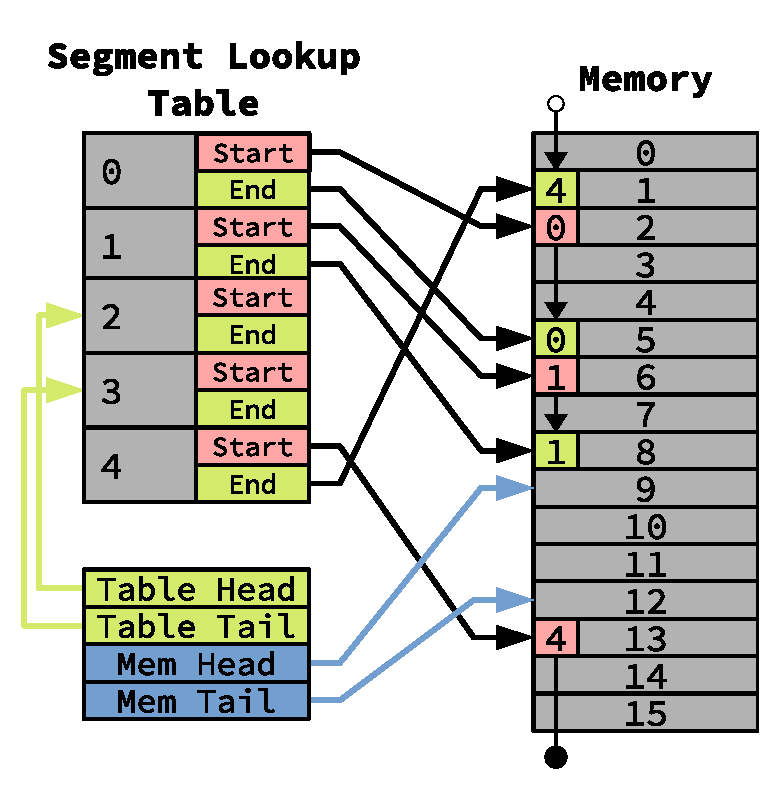
\includegraphics[width=\linewidth]{implementation/memory_segments.eps}
	\caption{The general structure of the memory segments in use.}
	\label{fig:memory_segments_explained}
\end{figure}

\subsubsection{Multi memory segments}
Each segment has three states, indicated by two boolean values; \texttt{Done}
and \texttt{Full}. When none are true, the segment is currently being filled
with data. When it is filled, and ready to be read, filled is marked as true,
and the data can now be read from. When the reading has ended, both \texttt{Done}
and \texttt{Full} are set to true, and the segment is now ready to be reused in
the lookup table. See \autoref{tab:memory_states_multi}.
\begin{table}[htpb]
  \begin{center}
      \begin{tabular}{l|c|c|}
          & \tablerot{\texttt{Full}}
          & \tablerot{\texttt{Done}} \\\hline
          \texttt{Filling}  &            &            \\ \hline
          \texttt{Reading}  & \checkmark &            \\ \hline
          \texttt{Done}     & \checkmark & \checkmark \\ \hline
      \end{tabular}
  \end{center}
  \caption{The memory states of "Multi memory segments"} \label{tab:memory_states_multi}
\end{table}
To describe the operation of the memory module, all the interface functions
are listed, and their operation explained.
The memory segment interface consists of the following functions:

\begin{description}
  \item[\csharpinline{int AllocateSegment(int size)}]\hfill\\
  When a segment is allocated, the new data is saved in the segment table
  head by looking at the \texttt{Table Head} pointer.\\
  The start and end pointers are calculated based on the \texttt{Mem Head}
  pointer. If the range between \texttt{Mem Head} and \texttt{Mem Tail} is
  smaller than \csharpinline{int size}, -1 is returned, indicating
  error. If not, the segment table id is
  returned(\csharpinline{int seg_ID}).

  \item[\csharpinline{int FocusSegment()}]\hfill\\
  A segment is classified as a focus segment if the data is ready to be sent
  (\texttt{Reading} state). It will automatically find the next segment, by
  incrementing the pointer by one, and if needed wrapping back to 0. The
  \texttt{Table Tail} is also moved by this action, to always point on the first
  instance of an active segment.

  \item[\csharpinline{int SaveData(int seg_ID, int offset)}]\hfill
  Returns the memory address for that specific segment with an offset.
  This is calculated by finding the start address in the segment table, and
  adding the offset. If the segment is not in "Saving" state, an error
  is returned of -1.

  \item[\csharpinline{int LoadData(int seg_ID, int offset)}]\hfill
  The same as \csharpinline{int SaveData(...)}, with the exception
  that an error is returned if we are not in the loading state.

  \item[\csharpinline{int DelaySegment(int seg_ID)}]\hfill\\
  This function delays a focus segment by copying it to the table head, and
  freeing the current \csharpinline{int seg_ID}. When this happens, the
  chronological order of the segments gets mixed.\\
  It is now impossible to tell if the next segment in the segment table contains
  the actual continuation of the memory. The next segment may be out of order,
  and point to memory anywhere. To get around this, each block gets an
  incremental ID at creation time. Since the creation of blocks always uses
  memory from the range \texttt{Mem Head} to \texttt{Mem Tail} the memory must
  be consumed in order.

  \item[{\pbox[c][1.7\baselineskip][b]{\linewidth}{{\csharpinline{void SaveMetaData(int seg_ID, MetaData meta)}}}}]\hfill

  Saves the \csharpinline{MetaData} into the current segment.

  \item[\csharpinline{MetaData LoadMetaData(int seg_ID)}]\hfill\\
  Loads the \csharpinline{MetaData} from the current segment.

  \item[\csharpinline{void SegmentFull(int seg_ID)}]\hfill\\
  Returns if the segment is \texttt{Full}.

  \item[\csharpinline{void SegmentDone(int seg_ID)}]\hfill\\
    Returns if the segment is \texttt{Done}
    %\notemark{Mener du "Done" her?}(See \autoref{tab:memory_states_multi}).

  \item[\csharpinline{int AllocateSegment(int size)}]\hfill\\
  Allocates a segment by getting the first available from \texttt{Table Head}.
  Returns the \csharpinline{int seg_ID} if a space is available.
  If none are available, return -1.
  %\notemark{Retur hvad?}
\end{description}




\subsubsection{Single memory segments}
The single memory segments are a bit different compared to the multi segments.
The single segments does not return an \csharpinline{int seg_ID} at any point,
because the focused segments are controlled internally. This is done to limit
the complexity for of the model, and to insure that segments are not accessed
out of order. Knowing and keeping the order makes it possible to allocate
segments without knowing the size beforehand.\\
The internal segment control
consists of three pointers. A pointer for the segment that is currently being
saved to, a pointer for the segment that is currently being read from, and
a pointer to the next segment ready for allocation.\\
This model is used as the internal buffers(see \autoref{subsec:memory_types}).
This requires that the metadata can be saved before saving the data.\\
Since segments in this implementation have undefined length before being marked
as \texttt{Full}, only one segment can be filled at a time. To save metadata,
the "allocation" method from "Multi memory segments" are reused. Instead
of giving the size of the segment, the metadata is given. This marks the segment
as \texttt{Active}. An \texttt{Active} segment is ready to receive data, but only
when the currently receiving segment is done filling. See
\autoref{tab:memory_states_single} for the different states.\\

\begin{table}[htpb]
  \begin{center}
      \begin{tabular}{l|c|c|c|}
          & \tablerot{\texttt{Full}}
          & \tablerot{\texttt{Done}}
          & \tablerot{\texttt{Active}} \\\hline
          \texttt{Inactive}
          %\tablefootnote{Internal state only used to detect if too many
          %segments are allocated, filling up the segment table.}
                            &            &            &            \\ \hline
          \texttt{Filling}  &            &            & \checkmark \\ \hline
          \texttt{Reading}  & \checkmark &            & \checkmark \\ \hline
          \texttt{Done}     & \checkmark & \checkmark & \checkmark \\ \hline
      \end{tabular}
  \end{center}
  \caption{The memory states of "Single memory segments"} \label{tab:memory_states_single}
\end{table}
%\noteimprovement{Maybe add stuff like }


\subsection{Dictionary} \label{subsec:dictionary}
%\notemark{It it not a sparsly linked list, but an sparse array implemented by a linked list}
The dictionary is used to keep track of out of order memory segments.
It works by keeping two tables, one for the keys and one for the actual values.
In this model, contrary to the memory buffers, the value table actually exists
since each value needs additional data. \\
The list implementation uses a linked list, where each element consists of an
offset to the next element, and an pointer to the next element. This is used to
represent a sparse array, where only actually valid elements are saved, and
anything in between are indicated by the offset.
 In the example in
\autoref{fig:memory_dictionary_explained}, The first key "0" consists of indexes
$(1,3,5,10)$, where their respective values is saved in
addresses $(0,3,1,4)$. As an example,
if the code requests index 5 of the linked list, address 1 is returned. If an
non existing index is requested, before being inserted , -1 is returned.
\begin{description}
  \item[\csharpinline{bool New(int key)}]\hfill\\
  When a new key is created, the key table is iterated over until a free element
  is found. If all are already used, false is returned.

  \item[\csharpinline{bool Free(int key)}]\hfill\\
  Removes a key and deletes and resets the values in their table. This will
  worst case iterate over all elements in the value table.

  \item[\csharpinline{bool ContainsKey(int key)}]\hfill\\
  Test if the key table have the key.

  \item[\csharpinline{int GetFirstValue(int key)}]\hfill\\
  Returns the first value of a key element. Finding the key in the key table takes
  n tries, but finding the first element takes constant time.

  \item[\csharpinline{int ListLength(int key)}]\hfill\\
  Get the length of the list with the offsets included. For example in
  \autoref{fig:memory_dictionary_explained}, the length of the list in
    key "0" is 10. This is calculated by adding all
    the offsets together from the key table, to the last element in the
    value table, with a pointer of -1.
    %\notemark{Markeret af Carl. Jeg kan hellere ikke helt se det fra tabellen...}

  \item[\csharpinline{int Insert(int key, int index)}]\hfill\\
  The insert creates a new entry in the value table. If it already exist, the
  same address is returned. If not, a new is returned. \\
  If a new value entry is returned, a free is found in the value table.
  The element before and after in the linjed list is found , and the new element
  gets injected between those.

  \item[\csharpinline{int Delete(int key, int index)}]\hfill\\
  Delete finds the element in the list and clears it up. If none are found, -1 is
  returned. The entries in the value table before and after the deleted element
  are merged together by changing the offset and pointer in the before entry.


  \item[\csharpinline{int Observe(int key, int index)}]\hfill\\
  Observe just returns the address if it exists, or -1 if not.

  \item[{\pbox[c][1.7\baselineskip][b]{\linewidth}{{\csharpinline{void SaveMetaData(int key, MetaData meta_data)}}}}]\hfill

  The keys have space for metadata, that can be loaded and saved.

  \item[\csharpinline{MetaData LoadMetaData(int key)}]\hfill\\
  Load the metadata.

\end{description}

\begin{figure}
	\centering
	\includegraphics[width=\linewidth]{implementation/memory_dictionary.eps}
	\caption{The general structure of the memory dictionary in use.}
	\label{fig:memory_dictionary_explained}
\end{figure}



\subsection{Memory types}  \label{subsec:memory_types}
Block ram on FPGA chips from companies such as Xilinx have a low latency, high
throughput but low capacity.\cite{xilinx_fpga_memory_resources}
The capacity limitation is a problem. Worst case the
system would have to hold multiple packets of the maximum size for that specific
protocol. For example, an \gls{ipv4} packet may have an max size of 65,535
bytes.\cite{RFC0791} If a lot of packets accumulate in the system, or the user
rarely empties the \texttt{Data In} buffer, we may run out of memory.\\
An additional solution would be the to use external memory with high latency
and high capacity. The throughput would have to be equal
or bigger than the stream from the system itself to not be an bottle
neck. For example, the DDR3 ram on the
TUL PYNQ\texttrademark-Z2\cite{tul_pynq} FPGA module could be used as external memory.
This memory have a max bandwidth of 1050Mbps, which would be a bottleneck
at 10 or 100 Gbps connections. The latency of these modules are also higher
than the internal block ram.
%\notemark{DDR3 paa Pynq boarded er 1050Mbps}\\
In both cases, the memory takes at least one clock to get results back from
memory. To guarantee that the data is available as soon as possible
(see: \autoref{sec:interface_signal_protocol}) one must use prefetching of the
memory.\\
This is solvable by using small internal buffers that use the fast registers.
The size of these small buffers would be based on the latency between the
request and response from memory. This would make it easier to
replace the underlying memory, by simply increasing the buffer size to that
of the memory latency.
%\notechange{Talk about how metadata is needed before the data itself}


\section{Interface Signal protocols}
\label{sec:interface_signal_protocol}
With the introduction of buffers between each parsing processes, a clear pattern
emerged. The layer-handling, "computing", processes are responsible for numerous real-time tasks
(parsing, sending, protocol-specific tasks, etc), while also limited by their
fixed internal buffers. These processes are not always ready to receive input
from preceding processes, while they at the same time must be able to write their
output to following processes immediately.\\
The buffers are a stark opposite, as their large internal block memories enable
them to buffer huge chunks of memory, while also being able to wait for the
succeeding process to start reading.\\
With these two established scenarios, protocols for each can be proposed -- the
Buffer-Producer protocol, and the Compute-Producer protocol.

\subsection{Buffer-Producer}
The Buffer-Producer (BP) is the interface signal protocol where the producer of
the data is a buffer process (such as \texttt{Data Out} or \texttt{Segment
Out}).\\
The Buffer-Producer is heavily inspired by the Transfer signalling protocol in
the AXI4-Stream standard, which ensures a two-way flow-control mechanism for both
the producer and the consumer\footnote{The producer and consumer are called
master and slave respectively in the AXI4 specification.}\cite{arm_axi4}.

\begin{figure}[h]
\centering
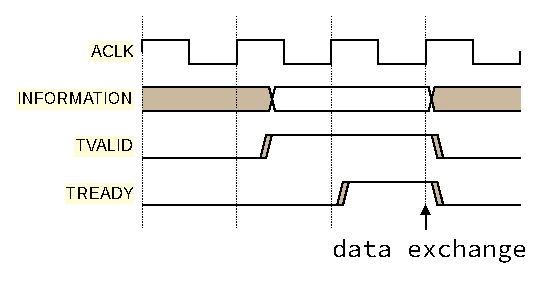
\includegraphics[width=\linewidth]{implementation/axi4_handshake.eps}
\caption{The AXI4 handshake process, adapted from “AMBA 4 AXI4 Stream-Protocol
	specification” by ARM, 2010, p. 19.\cite{arm_axi4}}
\label{fig:axi4_handshake}
\end{figure}

The AXI4-Stream protocol uses two signals (also called "flags"), the \texttt{TVALID}
on master, and \texttt{TREADY} on slave. Every time both \texttt{TVALID} and
\texttt{TREADY} are asserted during a clock-cycle, a data-exchange happens.
\autoref{fig:axi4_handshake} shows a data exchange, where the information
(the bytes) are placed on the bus and the \texttt{TVALID} is raised. When this
signal propagates to the slave, it asserts \texttt{TREADY}. When this signal
propagates back to the master, it knows that the information was read, and that
it can proceed with the next byte, or in this case, de-assert the
\texttt{TVALID} to indicate no more bytes available\cite{arm_axi4}.

The information transferred in the AXI4-Stream protocol is defined by the user,
as long as the width of the payload is an integer multiple of
bytes\cite{arm_axi4}.\\

The Buffer-Producer protocol draws heavy inspiration from this model, as it
provides a simple flow-protocol with only a few flags. However, the AXI4-Stream
protocol does not specify massive stream of data, where consecutive bytes are
sent on each clock-cycle. The issue is that, without any modifications to the
bare AXI4-Stream protocol, a producer will get notified of a value being read
by the consumer after 2 clocks. As shown on
\autoref{tab:axi4_stream_latency}, the producer has to wait 2 clocks before
updating the value on the bus, resulting in a clock in between transactions not
being utilized.


\begin{table*}[h]
  \begin{minipage}[b]{\dimexpr.5\textwidth-.5\columnsep}
    \centering
\begin{tabular}{p{1cm} | p{2.4cm} | p{2.4cm}}
\toprule
% \multicolumn{2}{c}{Item} \\
%\cmidrule(r){1-2}
		\textbf{Clock} & \textbf{Producer} & \textbf{Consumer} \\
\midrule
		0 & Puts data on bus and asserts \texttt{TVALID} &
		\texttt{TVALID} is low. NOP \\ \hline
		1 & \texttt{TREADY} is not set. Data from previous clock is
		kept on the bus & Reads data from bus and asserts \texttt{TREADY}\\ \hline
		2 & Observes that \texttt{TREADY} is asserted and updates the
		data on bus to next byte & \cellcolor{red!25} Still sees the
		old data from clock $0$!\\
\bottomrule
\end{tabular}
\caption{With the 2-clock latency for the \texttt{TVALID}/\texttt{TREADY}
	signal to propagate, the AXI4-Stream protocol cannot send consecutive
	bytes every clock.}
\label{tab:axi4_stream_latency}
\end{minipage}\hfill%
\begin{minipage}[b]{\dimexpr.5\textwidth-.5\columnsep}
\begin{tabular}{p{1cm} | p{2.4cm} | p{2.4cm}}
\toprule
% \multicolumn{2}{c}{Item} \\
%\cmidrule(r){1-2}
		\textbf{Clock} & \textbf{Producer} & \textbf{Consumer} \\
\midrule
		0 & Puts value on bus and asserts \texttt{TVALID} &
		\texttt{TVALID} is low. NOP \\ \hline
		1 & NOP & Sees that \texttt{TVALID} is high. Asserts
		\texttt{TREADY} but does not yet read the data from the bus.\\ \hline
		2 & Updates value on bus & Reads first byte \\ \hline
		3 & Updates value on bus & \cellcolor{green!25} Reads next byte \\ \hline
		n & Updates value on bus & \cellcolor{green!25} Reads n byte from the bus \\
\bottomrule
\end{tabular}
	\caption{By indicating a clock before about reading the value from the
	  bus, the 2-clock latency is avoided and the producer can update the
	  value on the bus every clock.}
\label{tab:bp_stream_latency}
\end{minipage}
\hrule
\end{table*}

This issue is circumvented in the BP protocol by asserting \texttt{TREADY} a
single clock prior, effectively indicating the intent of reading the value on
the bus during the next cycle. \autoref{tab:bp_stream_latency} shows that
even though it takes an additional clock to start a transaction, we can
circumvent the 2-clock issue that AXI4-Stream faces.\\

The BP protocol uses the same flags as those in AXI4-Stream, although slightly
differently. The \texttt{TVALID} flag is called simply \texttt{valid} in the
BP protocol. Likewise, the \texttt{TREADY} is called \texttt{ready}, however,
these both of these can be used interchangeably for clarity when comparing
against other protocols.\\

The final Buffer-Producer protocol can be summed up in these following
rules:
\begin{itemize}
	\item A data transfer only occurs a clock after both \texttt{valid} and \texttt{ready}
		are raised.
	\item When the producer has data available, it is immediately put in
		the bus and the \texttt{valid} flag is raised.
	\item Once the \texttt{valid} flag is raised, it cannot be reset until
		a data-transfer occurs.
	\item The consumer is allowed to wait until the \texttt{valid} flag is
		raised before raising the \texttt{ready} flag.
	\item If a consumer raises the \texttt{ready} flag, it is allowed to
		reset it before \texttt{valid} is raised.
\end{itemize}

The conventional data-exchange using the BP protocol in the network
stack is perhaps better visualized by a sequence diagram on
\autoref{fig:buffer_producer}.


\begin{figure}
	\centering
	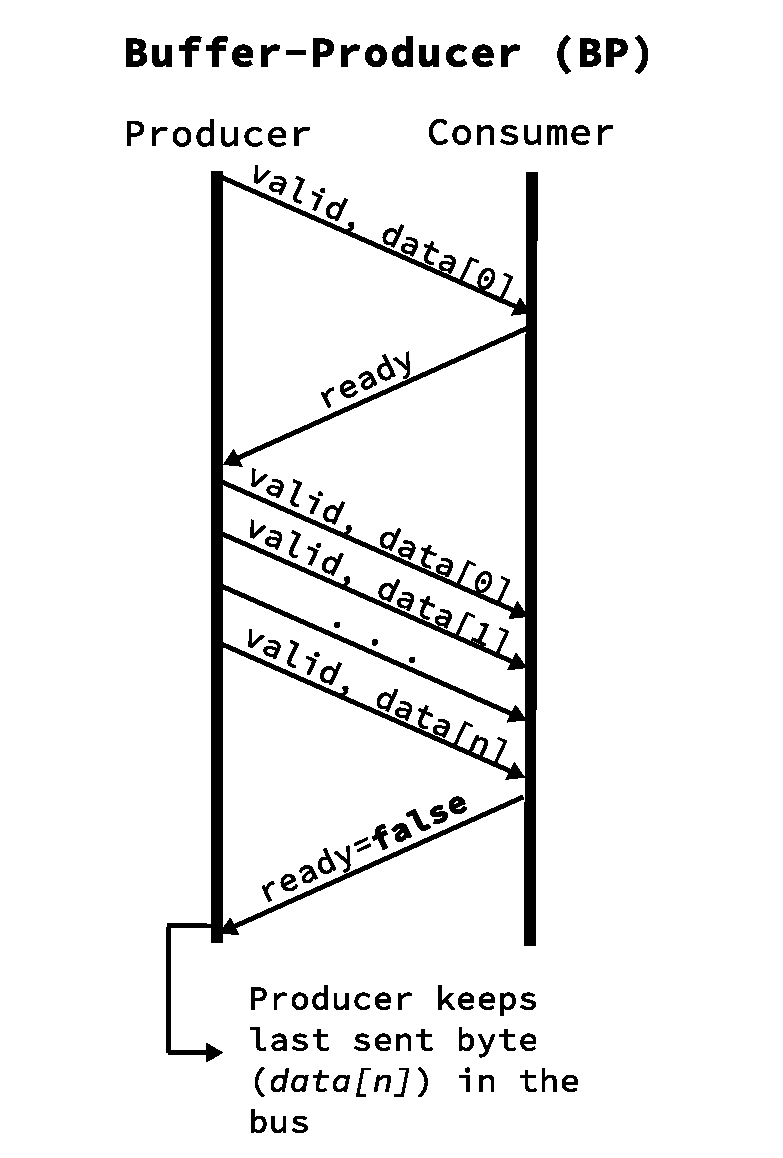
\includegraphics[scale=0.5]{implementation/buffer_producer.eps}
	\caption{The usual data-transfer between a buffer (Producer) and a
	compute-process (Consumer).}
	\label{fig:buffer_producer}
\end{figure}



\subsection{Compute-Producer}
The Compute-Producer (CP) protocol is the interface signal protocol from a
compute-process to a buffer. The requirement for this protocol is that
compute-processes do not usually have the luxury of being able to wait with the
data transfer, which usually happens if the compute-process is building a
packet header or passing information along from another buffer.

The concept for the Compute-Producer model is fairly simple; since the producer
(compute-process) does not have the luxury to wait, it always sends the data
on the bus, regardless if the consumer is ready. It is up to the producer to
mark the end of an ongoing data-stream.\\

Thus, the rules for the Compute-Producer protocol are as such:
\begin{itemize}
	\item If the producer puts data on the bus, the \texttt{valid} flag
		must be raised.
	\item If \texttt{bytes\_left} is greater than $0$, the data in the next
		clock will be valid.
	\item If \texttt{bytes\_left} is $0$, the current byte ends the
		current sequence of bytes.
	\item If the consumer deasserts \texttt{ready}, it \textit{may} not read the
		data in the bus.
	\item The producer may act upon the knowledge that the consumer is
		either reading (\texttt{ready = true}) or ignoring
		(\texttt{ready = false}) the data.
\end{itemize}

Such a scenario is visualized on \autoref{fig:compute_producer}, where the
consumer becomes unavailable during the transaction. The producer has the
opportunity to drop the transaction, but it might also continue till the end.

\begin{figure}
	\centering
	\includegraphics[scale=0.5]{implementation/compute_producer.eps}
	\caption{The usual data-transfer between a compute-process (Producer) and a
	buffer (Consumer). Note that the consumer becomes unavailable halfway through the
	transaction.}
	\label{fig:compute_producer}
\end{figure}



\section{Interface Control}
The \texttt{Interface} is a collection of 3 busses provided to the user. Two of
the busses are direct connections to the data-buffer, used to transfer the
actual data to and from the network. As seen on \autoref{fig:final_design}, the
connecting going to \texttt{Data In} follows the Compute-Producer interface
signal protocol, while the connection from \texttt{Data Out} follows the
Buffer-Producer protocol.\\
The connection going from the interface into the \texttt{Transport} process is
a bit more interesting. It is simply called the \texttt{InterfaceBus}, and it
is used to control the whole networking stack. As per usual, the connection
actually consists of a \texttt{InterfaceBus} controlled by the user, and the
\texttt{InterfaceControlBus}, used by the networking stack itself to respond to
the user requests.\\
Unlike the connection between buffers and processes where chunks of data are
transmitted over multiple clock-cycles, the interface connection is more of a
request-response model with only 1 clock-cycle required to submit the request
or send the response. However, after submitting the request, the user
\textit{should} keep the data in the bus until a response is received, because
the \texttt{Transport} process might be busy at the moment handling in- or
out-going packets, and not have time to process the request.\\
\autoref{fig:interfacebus_code} shows the definitions of the busses. Note
the \texttt{interface\_function} byte containing the type of "function" to
call, defined in the \texttt{InterfaceFunction enum} on
\autoref{fig:interfacefunction_code}.


\begin{figure*}[t]
    \centering

    \begin{subfigure}[b]{0.45\textwidth}
	\centering
	 %\begin{lstlisting}[language={[Sharp]C}]
\begin{mintedcsharp}
enum InterfaceFunction : byte
{
    INVALID = 0,
    // BIND = 1,
    LISTEN = 2,
    CONNECT = 3,
    ACCEPT = 4,
    CLOSE = 7,
    // ...
    OPEN = 255,
}

struct InterfaceData
{
    public int socket;
    public uint ip;
    public byte protocol;
    public ushort port;
}
\end{mintedcsharp}
%\end{lstlisting}

        \caption{Definitions of the structures used in the interface busses.}
	\label{fig:interfacefunction_code}
    \end{subfigure}%
\hfill%
    \begin{subfigure}[b]{0.45\textwidth}
	\centering
	 %\begin{lstlisting}[language={[Sharp]C}]
\begin{mintedcsharp}
interface InterfaceBus : IBus
{
    bool valid;
    byte interface_function;
    InterfaceData request;
}

interface InterfaceControlBus : IBus
{
    bool valid;

    byte exit_status;
    byte interface_function;
    InterfaceData request;
    InterfaceData response;
}
\end{mintedcsharp}
%\end{lstlisting}
	\caption{The definitions of the interface busses.\\\hfill}
	\label{fig:interfacebus_code}
    \end{subfigure}
    \caption{Pseudocode of the definitions used for the interface connection.}
	\label{fig:interface_definition}
\end{figure*}




\subsection{Usage}
The usage of this interface is very basic and primitive. The user sets the
appropriate values in the \texttt{InterfaceBus}, and raising the \texttt{valid}
flag. For example, to start listening on port $81$ using the \gls{udp}
protocol, the user would put the values on the bus as shown on
\autoref{fig:interface_request}.
\begin{figure}
\centering
\begin{Verbatim}[frame=single,samepage=true]
InterfaceBus {
  interface_function = CONNECT
  request {
    ip = 10.0.0.2
    protocol = UDP
    port = 81
  }
  valid = True
}
\end{Verbatim}
	\caption{A request on the \texttt{InterfaceBus} to connect to ip
	\texttt{10.0.0.2} using the UDP protocol on port 81.}
	\label{fig:interface_request}
\end{figure}


If the port is available under the \gls{udp} protocol and sockets are available
for allocation in the stack, the user should eventually receive a response.
On \autoref{fig:interface_response}, the user gets an \texttt{OK} response with the \texttt{socket = 2}:
\begin{figure}
	\centering
\begin{Verbatim}[frame=single,samepage=true]
InterfaceControlBus {
  valid = True
  exit_status = OK
  interface_function = CONNECT
  request {
    ip = 10.0.0.2
    protocol = UDP
    port = 81
  }
  response {
    socket = 2
  }
}
\end{Verbatim}
	\caption{A response to the request submitted in
	\autoref{fig:interface_request}. Socket "2" is returned.}
	\label{fig:interface_response}
\end{figure}
Once the user has received a valid socket, they can use the it at heart's
content for sending and receiving. \autoref{fig:interface_send_byte} shows
an example of sending the byte "A" to the newly created socket.
\begin{figure}
	\centering
\begin{Verbatim}[frame=single,samepage=true]
DataOut.WriteBus {
  socket = 2
  byte = "A"
}
DataOut.ComputeProducerBus {
  valid = True
  bytes_left = 0
}
\end{Verbatim}
	\caption{Sending the byte "A" to socket 2.}
	\label{fig:interface_send_byte}
\end{figure}
The user is not required to wait for any response, as the Compute-Producer
interface signal protocol is used.


\subsection{Limitations}
As briefly mentioned, a big limitation of the interface control is that only
one request can be proposed at a time, and the user has to wait an arbitrary
number of clocks before the response arrives. The issue is that the
\texttt{Transport} might be occupied processing in-going and out-going
packets.\\
To circumvent this, experimental features of creating a queue of requests in
the \texttt{Transport}-process was made. However, this only added complexity to
the code, increased the resource-consumption of the process by a large margin
just in order to maintain the queue data-structure, and apart from convenience,
it added no improved performance. For these reasons, the initial approach was
kept.













\chapter{Simulation}
\label{chap:simulation}

\chapter{Evaluation}
\label{chap:evaluation}

\noteinfo[inline]{Remember to describe that we could not get the network stack
down on the FPGA}
\section{Setup}
In the initial stages of testing, the components had simulation processes between
block. This made it possible to implement different blocks of the system
independent of each other.\\
These tests where changing a lot, because the initial design where not
reached yet.
When the modules where done, they where wired together and a simulator
where created to handle all input and output of the system.

\subsection{Graph file simulator}
\begin{figure*}[t!]
    \centering
    \begin{subfigure}[b]{0.16\textwidth}
        \centering
        \includegraphics[scale=0.45]{evaluation/graph_nodes/datain.eps}
        \caption{Data In}
        \label{fig:packet_graph_datain}
    \end{subfigure}%
    \begin{subfigure}[b]{0.16\textwidth}
        \centering
        
\includegraphics[scale=0.45]{evaluation/graph_nodes/send.eps}
        \caption{Send}
        \label{fig:packet_graph_send}
    \end{subfigure}%
    \begin{subfigure}[b]{0.16\textwidth}
        \centering
        \includegraphics[scale=0.45]{evaluation/graph_nodes/command.eps}
        \caption{Command}
        \label{fig:packet_graph_command}
    \end{subfigure}%
    \begin{subfigure}[b]{0.16\textwidth}
        \centering
        \includegraphics[scale=0.45]{evaluation/graph_nodes/dataout.eps}
        \caption{Data Out}
        \label{fig:packet_graph_dataout}
    \end{subfigure}%
    \begin{subfigure}[b]{0.16\textwidth}
        \centering
        
\includegraphics[scale=0.45]{evaluation/graph_nodes/receive.eps}
        \caption{Receive}
        \label{fig:packet_graph_receive}
    \end{subfigure}%
    \begin{subfigure}[b]{0.16\textwidth}
        \centering
        \includegraphics[scale=0.45]{evaluation/graph_nodes/wait.eps}
        \caption{Wait}
        \label{fig:packet_graph_wait}
    \end{subfigure}%
    \caption{The different node types in the simulation graph}
    \label{fig:packet_graph_nodes}
\end{figure*}%
The graph simulator is an abstract structure for easily composition and
illustrations of simulations in the system. The system can be boiled down
to inputs(sources) and output(sinks). The code is deterministic, since the same
combination of input and output signals would result in the exact same internal
state of the system. This means that a simulation of the system as a whole would
require knowing what to write/read at every source/sink, and doing it at the
right time. However, we do not need the timing on a clock to clock basis, since
the external network does not care when the system sends out a packet, only
if the packet is structured correctly. The user however may need information
regarding the latency of the system. The latency is based on the
specific system state, and is described in
\autoref{subsec:latency}.\\
With these assumptions it is possible to illustrate the timeline of the packets
with a graph, where a vertex does action on a clock to clock basis(etc. sending a
packet into the system.), and each edge describes what node to proceed to.
Each vertex have a state. When the \texttt{Valid} state is reached
the next vertex is set to the \texttt{Ready} state, but only if
they are connected via an edge. If a vertex contains multiple ingoing edges, each
vertex with outgoing edges to that vertex needs to be \texttt{Valid}.\\
{\renewcommand{\arraystretch}{1.3}
\begin{table}[htpb]
    \begin{center}
        \begin{tabular}{lcl}
            State & Color&Description\\ \hline \hline
            \texttt{Dormant}& \statecolorbox{graph_dormant} &
            \makecell{Vertex is not in use.}\\ \hline

            \texttt{Ready}& \statecolorbox{graph_isready} &
            \makecell{Vertex Is ready\\ for activation.}\\ \hline

            \texttt{Active}& \statecolorbox{graph_active} &
            \makecell{Vertex is active.\\ Simulator is\\ gathering data.}\\ \hline

            \texttt{Inactive}& \statecolorbox{graph_inactive} &
            \makecell{Vertex is inactive.\\Simulator is not\\ gathering data.}\\ \hline

            \texttt{Valid}& \statecolorbox{graph_valid} &
            \makecell{Vertex is done\\ and validated.}
        \end{tabular}
    \end{center}
    \caption{The different states of the nodes, and their respective colors} \label{tab:graph_node_states}
  \end{table}
}\\
Each vertex have their own type, defining what input source or output sink to
use. The graph file simulator consists of multiple input sources and output sinks
as seen in \autoref{fig:packet_graph_nodes}.\\
There are three inputs, giving data to the system:
Data in(\subref{fig:packet_graph_datain}),
Send(\subref{fig:packet_graph_send}) and
Command(\subref{fig:packet_graph_command}).
There are two sinks, getting data from the system
Data out(\subref{fig:packet_graph_dataout}) and
Receive(\subref{fig:packet_graph_receive}).
The node type Wait(\subref{fig:packet_graph_wait}) is special, since
it does not use a input or a sink. It simply counts down each clock, until it's
counter reaches zero.\\
Since there only exist one of each input source and output sink (except Wait),
the simulator can only work on one vertex of each type at a time.
In graphs where there are multiple ready vertexes of same type, the vertex with
the lowest ID are focused on first. When a vertex is focused, it is set as
\texttt{Active}.
\\\\
As an example of this graph, see \autoref{fig:graph_simulation_running_examples}.



\begin{figure*}[htpb]
    \centering
    \begin{subfigure}[b]{0.5\textwidth}
        \centering
        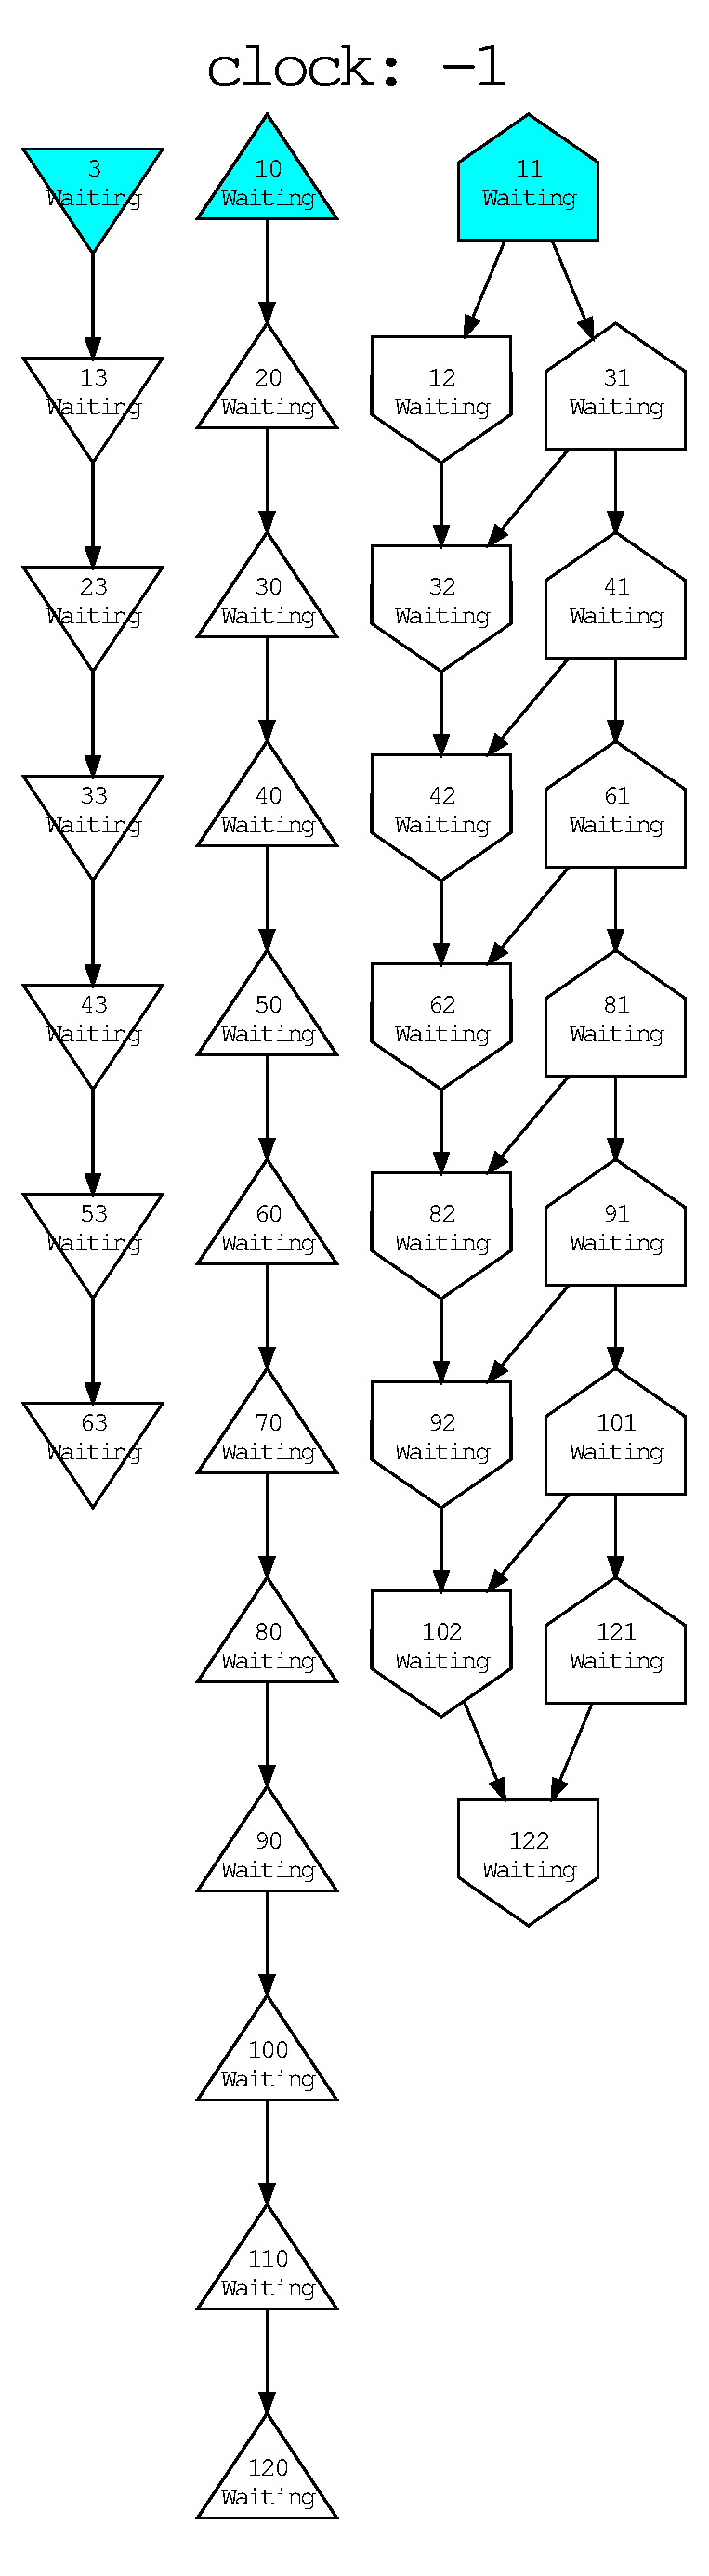
\includegraphics[scale=0.45]{evaluation/example_graph_initial.eps}
        \caption{The initial state of a simulation}
        \label{fig:example_packet_graph_initial}
    \end{subfigure}%
    \begin{subfigure}[b]{0.50\textwidth}
        \centering
        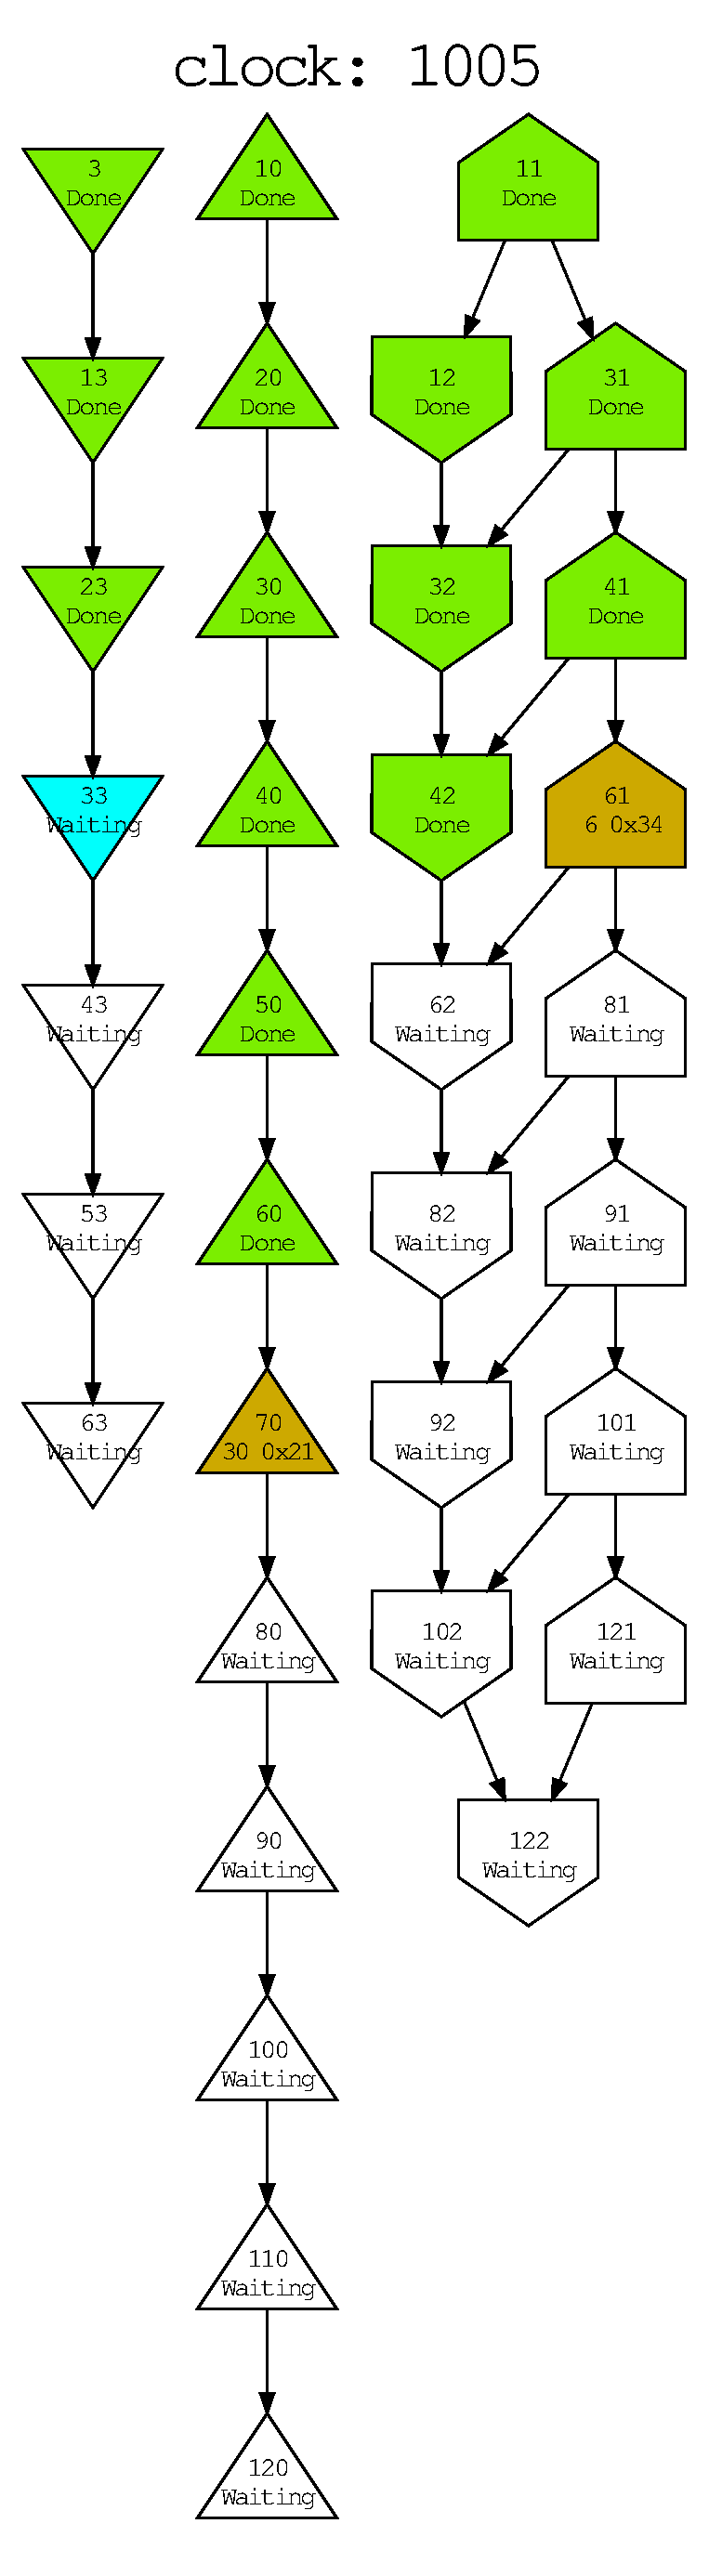
\includegraphics[scale=0.45]{evaluation/example_graph_running.eps}
        \caption{The state after 1005 clocks}
        \label{fig:example_packet_graph_running}
 	\end{subfigure}%
    \caption{A Illustration of the graph states before running and 1005 clocks
    inside the simulation}
    \label{fig:graph_simulation_running_examples}
\end{figure*}



\section{Test}
\subsection{Latency}\label{subsec:latency}

\section{Verification}

 % Rename this to "Verification" for FPGA lingo?
\chapter{Discussion}
\label{chap:discussion}
The intent of this project was not only to implement an efficient, high-speed,
and responsive TCP/IP stack, but also to test the viability of \gls{sme} for
this types of projects. In this chapter, the results from the tests are
investigated, the viability of the networking stack is discussed, and the usage
of SME for this project is examined.

\section{Compiling to hardware}\label{sec:compiling_to_hardware}
Since the \gls{sme} vhdl code generator never converted the project. It is hard
to comment about the codebase working on hardware.\\
However, we did notice a problem in \autoref{subsec:dictionary} regarding
the dictionary implementation. To find a value in the value table, it may have
to traverse the same table multiple times in random order. This means that the
value list would be iterated over at most $n$ times. In each iteration there are
$n$ branches. The total amount of branches for the operation is therefore $n^2$.
In the current design, this happens in one clock. This would result in a very
long path with multiple lookups, multiplexers and number operations in one clock.
This is not ideal, and would possibly be the slowest and biggest
component in the system.\\
A possible solution is discussed in \autoref{subsec:bug_dictionary_lookup}


\section{Performance}
In the test chapter \ref{chap:evaluation}, we ran the simulation for
multiple hours. In about 2 million clock cycles, the networking stack was able
to handle 17283 packets in total, where 1280 of the packets were valid
connections intended for the user of the stack. During the test, the valid
data-stream was also sent out in identical 1280 packets.\\ % \notemark{Fix!}
If the network stack was clocked at a very modest clock-rate of 10 MHz of the
maximum 866 MHz on the Xilinx Zynq-7000 series\cite{xilinx_zynq_7000}, the
network is theoretically able to run at:
$$1\:\mathbf{Byte}*10\:\mathbf{MHz}= 80\:\mathbf{Mbps}$$

This speed is by no means exceptional, in fact, it is very slow compared
to even common ethernet network adapters found in consumer server hardware, such
as the Intel Ethernet I210 series\cite{intel_1gbps_nic}.\\

However, the network stack never reached the actual hardware, so the
theoretical speed is questionable. Furthermore, since the most resource-heavy
processes cannot be investigated, optimization of the stack would be premature
as of now.


% 118400 packets in total
% 1280 ingoing
% 1280 sent
% clocks: 10 000 000 mio.


\subsection{Improving performance}


\begin{figure}
\centering
\includegraphics[scale=0.45]{discussion/design_stacked.eps}
\caption{Replicating the "inner" part of the design in order to multiply the
performance. }
\label{fig:design_stacked}
\end{figure}


Even though many optimizations can be done on the network stack codebase
itself, there are other ways of achieving better performance from the project.

\subsection{Increasing the throughput by widening the data channel in the
busses}
Perhaps the most instinctual way of improving the performance of a network
stack is by increasing the throughput. By increasing the width of the
\texttt{data} channel in the buses carrying information, the throughput could
potentially increase manyfold.

While this change is perfectly doable in the hardware and easy to implement in
the code, it might also have some unexpected consequences on the logic of the
processing modules.

For example, while not strictly a requirement, most, if not all, header sizes
are a multiple of 8 bits. By transferring only 1 byte at a time, the system is
sure to never cross the boundary of a header in the same clock cycle. If,
however, the data-bus transferred 2 bytes at a time, the first byte might be
the last part of a header, while the next byte is a data-byte. In that case,
the process has to not only parse the finished header, but also forward the
second byte down to the next process. Here again will the processes need
additional logic needs to check how much of the data-bus actually contains
valid data. Figure \ref{fig:bus_width_boundaries} illustrates the problem of a
data-segment not aligning with the bus-width.

\begin{figure}
\centering
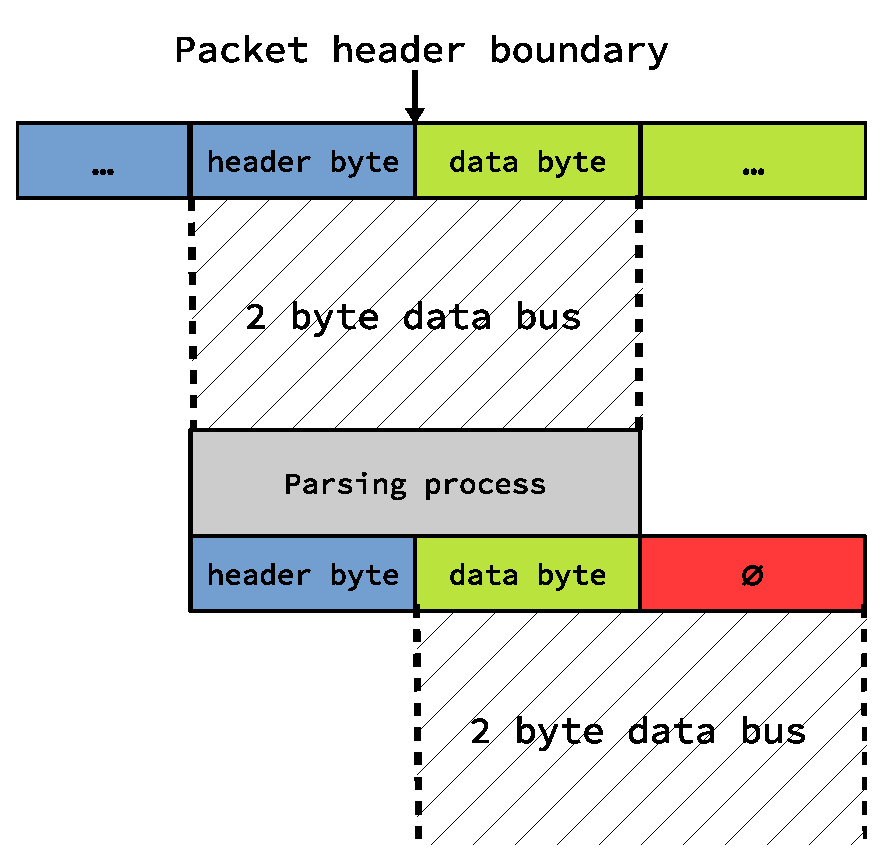
\includegraphics[scale=0.45]{discussion/bus_width_boundaries.eps}
\caption{the design in order to multiply the
performance. }
\label{fig:bus_width_boundaries}
\end{figure}





\subsection{Replicating the system}
During the design-phase, it was important to ensure the active connections
arrived on the same stack, since the IP fragments have to be collected on the
same buffer, and the TCP state has to be synchronized.

The \texttt{Transport} is especially burdensome, as it has to handle both
ingoing- and outgoing-packets, as well as the user interface calls and
protocol-specific handshakes and other operations. Finding a way of getting
around this congestion, it should be possible to parallelize the system for
better performance.

By replicating the networking stack and assign a unique IP address to each, it
should be possible to create a "Load Distributor", distributing the packets
across multiple networking stacks. Figure \ref{fig:design_stacked} shows a
prototype design, where the inner part of the networking stack is duplicated on
the FPGA itself. The \texttt{Load Distributor} conveys the packets to the
appropriate network-stack.

On the other side of the same figure, the \texttt{Load Collector} ensures that
the replicated network stacks work as one, and that they are abstracted away
in the \texttt{User Interface}, so that the user does not have to make up for
the separation. Even though the \texttt{Transport} processes do not share any
information across the stacks, they can have hardcoded \texttt{socket} numbers,
assigning a block of sockets to each stack, so that overlap does not happen.


\section{Usability}
Perhaps the most important aspects of any software project is its usability,
versatility, and its application.
While it is shown in chapter \ref{chap:evaluation} that the networking stack
performs arguably well in a reasonable simulated scenario, it is to be seen
whether the project can bring any value to the user.

\subsection{Intended usage}
The intended usage of the networking stack is to be integrated with existing
FPGA hardware in order add networking capability to a system. These systems
range from simple embedded \gls{iot} devices to large \gls{nic} cards.\\
Although it is possible to connect an SME project with other VHDL projects, it
is much more straight-forward to add the networking code directly into an SME
project.\\
For instance, other SME projects, such as the "High Throughput Image Processing in X-ray
Imaging" developed by Troels Skjøttgaard Ynddal\cite{troels}, which does
real-time image processing on x-ray images, could benefit from a network stack
by sending the processed images to a server for further analysis and backup.

\subsection{Existing solutions}
Sadly, the developed networking stack could not be brought onto an \gls{fpga},
making the comparison to existing solutions difficult.
In theory, if the networking stack worked on an FPGA, it would bring little to
no runtime advantages over existing FPGA TCP/IP stacks, such as the
Xilinx 10Gbps TCP/IP Stack\cite{sidler2016lowlatencytcp}.
However, the networking stack is easily extensible and modular. The design
choices made during the development have proven to make the stack very flexible,
and the programmer can easily add or remove protocols. The use of the C\#
programming language makes it more accessible for software engineers to modify
the code without prior knowledge to the hardware itself, or special \gls{hls}
tools and languages, albeit without the dynamic constructs of the C\# language.


\subsection{Integration with existing hardware}
As an extension to this project, the code for the Digilent Pmod NIC100\cite{pmod_nic100}
has been developed by Carl-Johannes Johnsen to act as the \texttt{Link Interface}
\cite{carl_pmod_nic100}, so that the networking stack could be tested on real
hardware.
While the stack never reached bare-metal, the testing suite simulates this
connection from the Pmod100 into this \texttt{Link Interface}. Although testing
on real hardware has to be carried out for definitive results, the simulation
suggests that this connection with networking hardware can indeed work.


\section{Using C\# with SME}
Not only had the use of C\# with \gls{sme} a great impact on the design, but the
whole project as a whole.

\subsection{Concurrency}
As was the intent of the \gls{sme} project, the messaging framework was
indispensable during the development of the networking stack. Besides not
having to concerns ourselves with the synchronization across processes, the
"Shared Nothing" property of \gls{sme} was a great help during the design, and
forced the design to be neatly isolated in the appropriate layers.

The isolation of each \texttt{Process} object gave a great overview of what each
"thread" of the system was doing. Likewise, the information exchange was very
clear, since it was nicely collected in one place -- the bus.

Sadly, the parsing of network packets is excessively sequential, and the
project does not utilize the full potential of SME in that regard.

\subsection{Cumbersome initialization and alternation}
% Parallelism hard from software
% Initialization of busses is cumbersome
The way projects are written in SME with C\#, the programmer has to
choose a design hardware architecture beforehand, since adding new SME
processes after the fact is cumbersome, and requires a lot of manual
modifications.
For instance, injecting a new process in between two existing processes
requires potentially adding new busses to the system and set these up correctly
in the code. Although this is a trivial task, the process itself is prone to
typos and oversights from the programmer.


\subsection{Using the C\# language}
In the beginning, it was pleasant to use a familiar language for the
implementation of the networking stack. Yet, as the code-base grew in size, the
flaws started to surface.

The C\# programming language is a very actively developed language with many
modern features, it is widely used with a very active community, and it has a lot
of useful packages and frameworks.

When writing code for the simulation, all of these utilities and features can
be used, providing the programmer with endless possibilities for
simulation-scenarios. For instance, inn this system, the simulation processes use the
file-system to load pre-recorded packets and feed them into the
simulation or to create log-files of the simulation\footnote{
A number of experiments have also been carried out in order to replace the
native networking stack with the simulation}.

Unfortunately, almost none of these features are available with \gls{sme}
when writing code for the FPGA, as most of these require dynamic constructs,
such as instantiation of new classes or use of dynamic collections. Although
this restriction is caused by the hardware and not \gls{sme} itself,
the C\# language started to be much less intuitive. Instead of applying
best practices and exploring new features in a well-known and established
language, we had to limit ourselves to the viable subset of the working
features, and create the design around it. While it is understandable why
a proven language is used to test out a new message passing framework,
the C\# language did not always feel right for hardware development, and
the upcoming \gls{smeil} might prove itself to be a welcome addition to
the \gls{sme} project.\cite{github_smeil}.


\subsubsection{Pre-written components and modules}
The \gls{sme} framework already contains premade objects for use, such as the
\texttt{TrueDualPortMemory}, which is a process that helps the programmer write
code interfacing with the built-in block memory on the \gls{fpga}.\\
As of yet, only a few memory components are included in the \gls{sme}
framework.

During development, there was a pattern of prevailing components and systems
reused in multiple processes:
\begin{itemize}
\item \textbf{Generic buffer process}\\
As documented in the design section, the buffers make up a big part of
functionality in the whole system. However, these \gls{fifo} constructs
are very commonly used during FPGA development\cite{fpga_fifo}. A generic
\gls{fifo} buffer component would be a very useful feature during the
development of the networking stack.

\item \textbf{AXI4 communication process}\\
In the processes, the programmer is free to implement any bus interface signal
protocol. Although a custom protocol was implemented for the system, it has
been cumbersome and challenging to implement two processes with a shared signal
protocol. Pre-written processes with support for established signal protocols
could be a valuable addition to the \gls{sme} ecosystem.

\end{itemize}


\subsection{Process state modelling}
Most processes in the system have multiple states, some containing fairly
complex state-transitions, as seen on figure \ref{fig:statemachines_internetin_transport}
in chapter \ref{chap:implementation}.\\
Introduced in the implementation chapter, \gls{sme} provides the
\texttt{StateProcess} class to simplify the creation of processes with
multiple states. This class proved itself to be immensely helpful in the
\texttt{Internet Out} process, which consist solely of sequential states.
Unfortunately, this construct is inadequate and incomplete to model the rest of
the computing processes, which were slightly more complex state-machines, as
those used in the system.

\subsubsection{Repeated code}
\begin{figure}
\centering
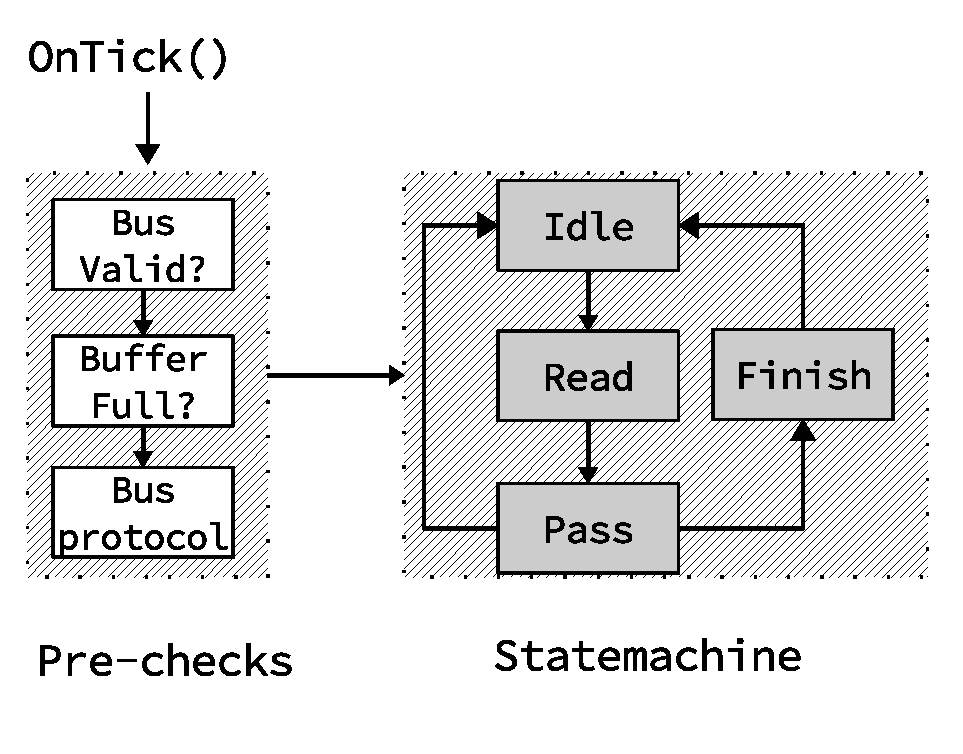
\includegraphics[scale=0.45]{discussion/fsm_prestates.eps}
\caption{An example of a process state-machine with pre-checks regardless of
the current state.}
\label{fig:fsm_prestates}
\end{figure}

The first identified issue was that most processes need to run certain checks on the
start of each clock cycle, such as checking the validity of the busses,
ensuring that there were no errors in the data-stream, maintain a bus signal
protocol, or make sure that some other limitations are met.
With the conventional \texttt{StateMachine}, this is intricate to write these
checks without much repetition. Instead, in this project, regular processes are
used in combination with an internal variable keeping track of the state.
This subtle difference lets the programmer have a unified entry-point to the
code, and branching code can be written to enter the appropriate
state-functions in the code.
For instance, figure \ref{fig:fsm_prestates} visualizes that a unified
pre-checks can be run prior to enter state-specific code. This adds a lot to
the length of the "code-path", but it avoids a lot of repetition in the code.


\subsubsection{Complicated state changes}\notejan{Spoerg Carl om hans kommentar}
Another common issue with modelling state-machines with \gls{sme} was certain
state-changes. In situations where a process is executing the last cycle of a
state that writes to some bus, a state-change is often desired in the end.
However, most state-transitions need to do some cleanup, for instance resetting
variables or re-initialize busses. If this cleanup happens in the same clock as
the last byte is written to the bus, this value will never arrive at the other
end. To circumvent this, the \texttt{Finish} state was utilized, which delays
the state-transition a single clock, giving the busses a clock-cycle window to
propagate correctly.

While this solution worked fine, the code itself was identical across processes
with this issue, and re-implementing was cumbersome and error-prone.

\subsection{Bugs and other lesser issues}
The\gls{sme} framework has been surprisingly stable, albeit with a few minor
bugs. Although most of these issues are being fixed at the time of writing,
they were still a noticeable hindrance during development:
\begin{itemize}
\item \textbf{Reserved VHDL keywords}\\
Certain words in the C\# code were reserved in\gls{vhdl}. While this is a
non-issue if the project is not being compiled to \gls{vhdl} code, this needed
to be taken into consideration during development. One such reserved word  was
the "Transport", used to denote the \texttt{Transport} process class.

\item \textbf{C\# structs}\\
A lot of information has to be passed between the buffers and processes. For
the sake of readability and maintainability of the codebase, this data is best
encapsulated in namespaces for a hierarchical organization.
Luckily, \texttt{struct}s became available shortly after the discovery of this
requirement, and are used in the project. For instance, the
\texttt{InterfaceBus} uses two of the \texttt{InterfaceData} struct.

\item \textbf{Slow simulation}\notejan{Naevn at det stadig kan vaere hurtigere
	end VHDL}\\
The tests carried out during the evaluation of the system were astonishingly
slow. While the simulation ran at an acceptable rate in the beginning, it
started slowing down as the test progressed. A simulation lasting multiple
hours only managed to simulate a few millions of clock-cycles.

\end{itemize}



\section{Discussion}

\begin{frame}
  \frametitle{Discussion}


\begin{columns}
\begin{column}{0.5\textwidth}

Estimated performance:
$$1\:\mathbf{Byte}*10\:\mathbf{MHz}= 80\:\mathbf{Mbps}$$
% \item<3>Usability
% \item<4>Using C\#
% \end{itemize}
\end{column}

\begin{column}{0.5\textwidth}

Improving the performance:
\begin{figure}
\centering


\includegraphics[scale=0.25]{../thesis/discussion/design_stacked.eps}
\end{figure}
\end{column}
\end{columns}
\end{frame}


\begin{frame}
\begin{columns}
\begin{column}{0.5\textwidth}
Usability

\end{column}

\begin{column}{0.5\textwidth}
SOMETHING
\end{column}
\end{columns}
\end{frame}

\begin{frame}
\begin{columns}
\begin{column}{0.5\textwidth}
Using C\#
\end{column}

\begin{column}{0.5\textwidth}
State modelling\\
Simulation\\
Concurrency
\end{column}
\end{columns}
\end{frame}

\section{Conclusion}
\begin{frame}
  \frametitle{Conclusion}

\begin{itemize}
\item Lot of trial and error to find the optimal design in the beginning
\item In 10 mio. simulated clock cycles, 17283 packets were handled,  1280 of
which were correctly received by the Application layer, and then sent out
again
\item Even with a few flaws, SME is a great framework for hardware modelling
\end{itemize}

\end{frame}

\chapter{Future work}
\label{chap:future_work}

\section{Bugs}
A few small bugs have been found during the test phase. While these are
described in the discussion test-chapter, here is a brief list:
\begin{itemize}
	\item \textbf{Destionation IP address not set}\\
	The destination address of the IPv4 header is not set in the outgoing
	packets. \texttt{Transport} is the source of this bug, as it does not
	set the appropriate field in the bus to \texttt{Segment Out}.

	\item \textbf{Protocol field not set}\\
		Just like the IPv4 destination address not being set in
		\texttt{Transport}, neither is the \texttt{Protocol} set.
\end{itemize}
However, the dictionary implementation (\autoref{sec:compiling_to_hardware})
is a show stopping bug, that needs a solution. Luckily, this can be fixed in
a way so the general flow of the system consists, and only simple changes have
to be made.

\subsection{Dictionary module solution}  \label{subsec:bug_dictionary_lookup}
The problem with the dictionary calculations was the exponential growth of
components needed based on the length of the value list. A solution would
be to split the calculations over multiple clocks. Since the loop needs to
traverse the value list multiple times, it would be ideal to split each iteration
of the initial loop into their own clock. This limits the amount of branching to
only $n$ per clock. This solution will create latency between the insertions and
reads of the array values. \\
\notemark{Finish!}

\section{Improvements}
Although the current implementation of the networking stack has enough
functionality to be useful in certain applications, there are a lot of
improvements that can be carried out in order to better the project.


\subsection{Wider data-channels between processes and buffers}
One of the main bottlenecks for the throughput is the raw amount of data the
networking stack is working with at any given moment. Currently, the channels in
the SME busses carrying data are only a byte wide, that is, at any given clock,
a process will only have at most 8 bits to work with.
This 1-byte width has been used because it is the most intuitive to work with,
as packet-header fields usually span a factor of 8 bits.\\
Extending the width of the data-channel in the busses might improve the
throughput manyfold, but it might also introduce more logic to the bit-shifting
and masking to parse the headers. Additionally, this change does not only affect
the parsing and the headers, but also the logic in the addressing for storage
in the buffers, as well as, for instance, the checksum calculation.

\subsection{Add external verification tool}
The tests performed and described in chapter \ref{chap:evaluation} on the
current implementation have shown no major nor breaking bugs or errors for
the supported subset of protocols in the internet protocol suite.
Since the existence of undiscovered bugs cannot be ruled out with the
custom-made testing suite, it is better to use an external verification tool in
order to not transfer any wrong implementation-details over to the
test-tools.\\
There are a multitude of ways to TCP/IP implementation with both regards to
bandwidth and throughput, stability, loss, etc.
One such tool is the \texttt{iperf3}, which is a "TCP, UDP, and SCTP network
bandwidth measurement tool"\cite{iperf3}. It is a highly efficient tool for
both performance test, but also verify the correctness of a networking stack.
By introducing the iperf3 testing suite as a means to test the implementation of the networking
stack, a much better insight of the correctess of the stack can be gained.


\subsection{Unsupported Transport protocol pass-through to Application layer}
Even though the networking stack should be easily modifiable, it is conceivable
that certain users would rather parse certain transport protocols directly in
"user-space" by reading raw transport segments from the interface.

This is a fairly common phenomenon to first test a conceptual protocol in
user-applications, and then implementing them in the appropriate layers. For
example, this is the reason why the Linux kernel provides raw packet reception
and transmission in the user-space directly from the kernel network
stack\cite[Version~Linux 5.3-rc6, \texttt{Documentation/networking/tuntap.txt}]{linux}.

While passing segments directly through \texttt{Transport} to the \texttt{Data
In} buffer, new functions need to be introduced in the interface busses to
enable the user to flag which connections need not be parsed.



\section{New features}
As discussed in chapter \ref{chap:design}, the networking stack is designed
with extensibility in mind, with a separation for the link-, the internet-, and
the transport-layer. Given a protocol following the classic internet protocol
suite 4-layer model, it should be possible to implement this protocol in the
networking stack without major changes to the underlying structure of the whole
codebase.\\
The implementation only supports \gls{udp} in the transport layer, which is
still a great streaming protocol for a multitude of viable scenarios. However,
situations where packet loss or out-of-order data-stream is not acceptable,
\gls{tcp} is the ideal choice of protocol to implement in the stack. With the
ability to share state across sockets in the \texttt{Transport} module, the
parser for the \gls{tcp} header can be implemented, and the out-of-order nature
of the incoming data is already handled in the \texttt{Data In} buffer.\\
Likewise, the newer version of the Internet Protocol, the \gls{ipv6}, is slowly, but
surely, seeing adoption on the internet. Fortunately, the protocol itself is
actually slightly easier to parse compared to its predecessor, the \gls{ipv4}.
For instance, multiple flags from the older \gls{ipv4} header have been moved
into the optional section of the \gls{ipv6}. Furthermore, fragmentation of
\gls{ipv6} packets have been restricted somewhat, and not all hosts are required
to support it\cite{ipv6_proposed}.



\section{Adding a firewall}
\begin{figure*}
\centering
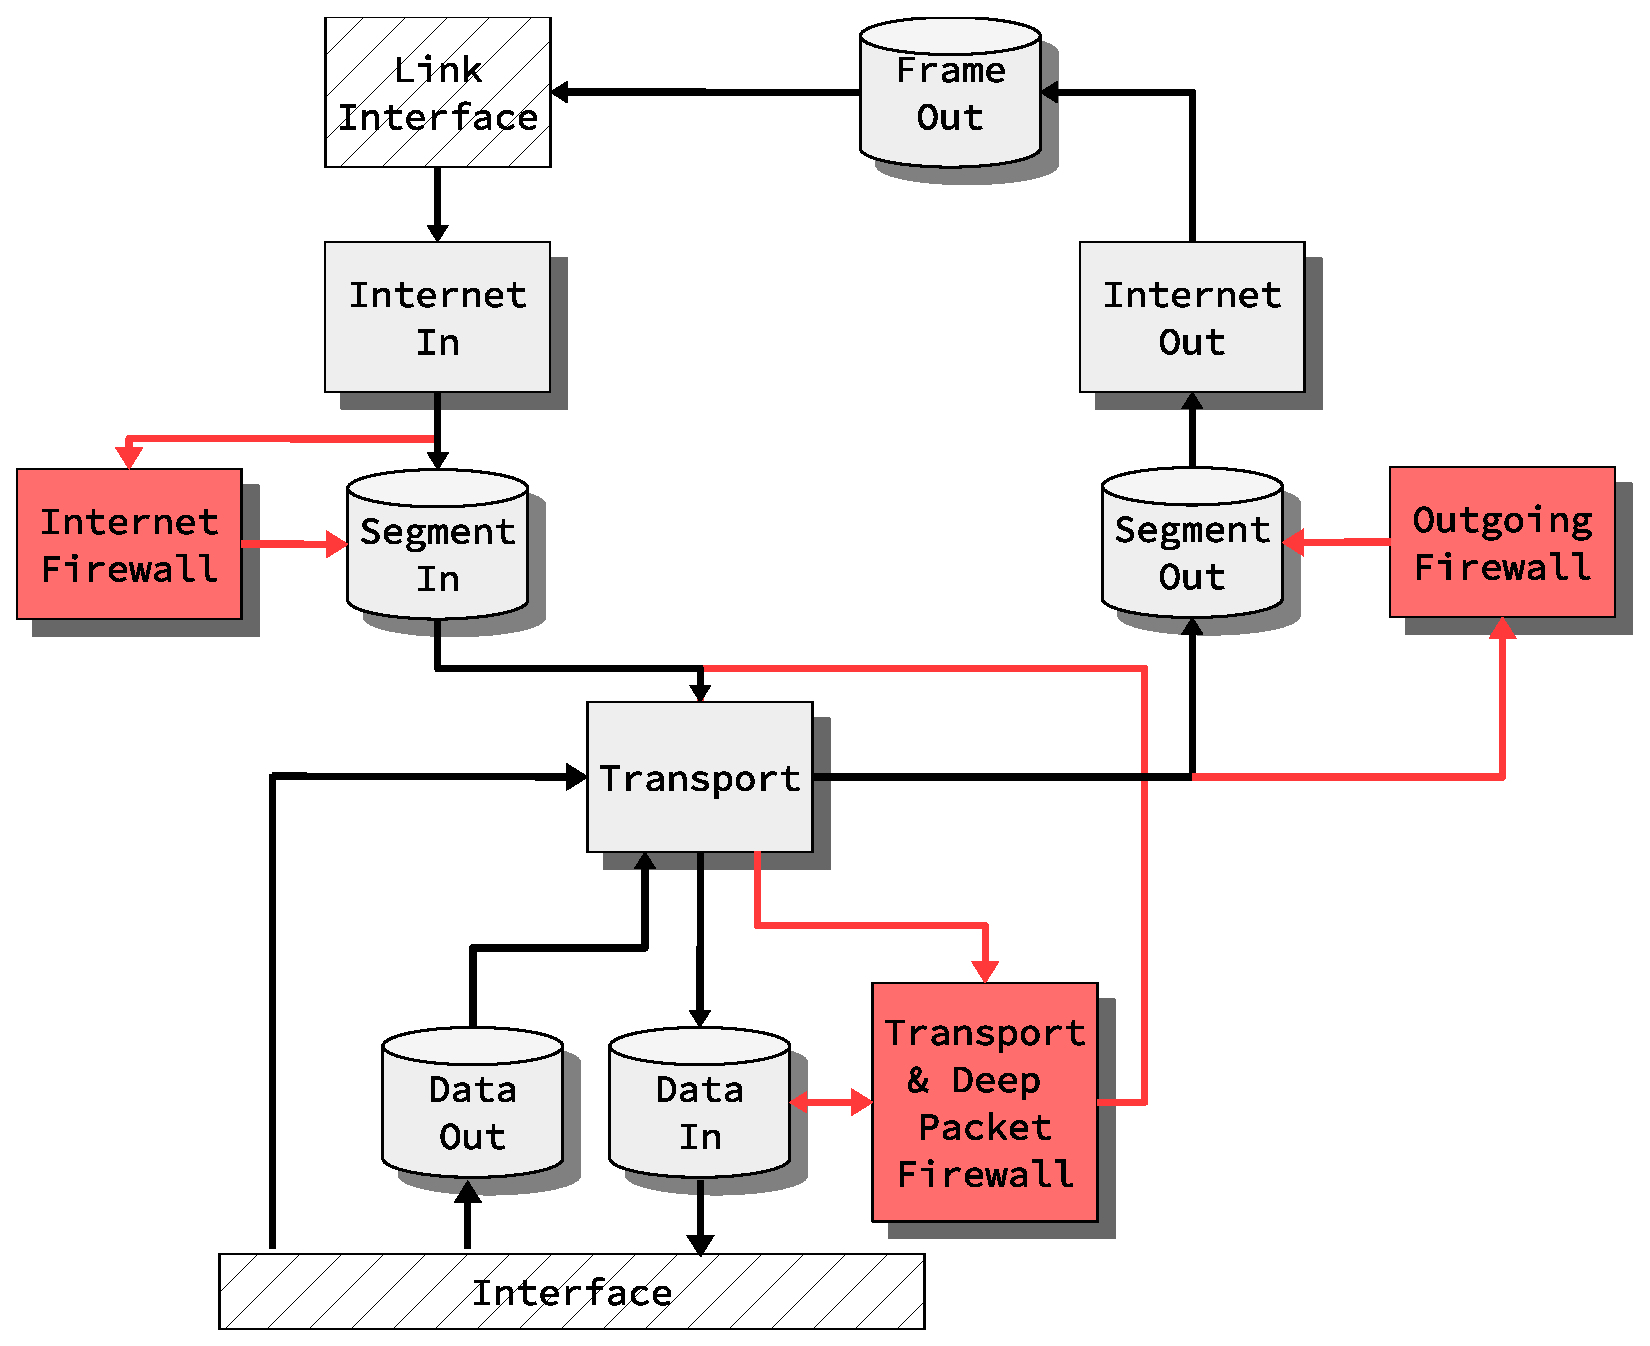
\includegraphics[scale=0.50]{future_work/firewall_integration_design.eps}
\caption{The proposed design for integrating the network stack with the
accompanying firewall}
\label{fig:firewall_integration_design}
\end{figure*}


In tandem with this project, a FPGA firewall has been developed by
Patrick Dyhrberg Sørensen and Emil Sander Bak. Just like the networking stack,
the firewall is implemented in \gls{sme}, with the intent to be easily
integrated with networking stacks, such as this one\cite{fpga_firewall}.\\
The firewall consists of whitelist rules, connection states, "deciding"
processes, and busses for communication and synchronization\cite{fpga_firewall}.\\
The processes making the actual decisions are split into 3 state processe:
\begin{itemize}
\item \textbf{Incoming IPv4}\\
The first point where the firewall can do any decisions is when the internet
protocol header is parsed. This header provides information such as the source
and destination address, and the firewall can do basic checks for blacklisted
or whitelisted addresses, as well as detecting some suspiciously formatted
packets.
\item \textbf{Incoming Transport}\\
The transport-part of the firewall is perhaps a bit more interesting. Here,
the firewall can not only check on the source and destination ports of a packet,
but also verify that there are no malicious intents with regards to the protocol
specification itself. For example, the firewall can detect and stop a SYN-flood
attack, which is a form of \gls{dos attack} where the attacker sends a large
number of TCP SYN-request to a host in order to consume all the host
computational resources.

\item \textbf{Outgoing}\\
The last point that the firewall monitors is the outgoing traffic. This is in
place for situations where the networking stack tries to communicate with
malicious or forbidden hosts.
\end{itemize}

\subsection{Proposal for the design of incorporating the firewall}
Although both projects have been designed to be combined with each other,
there have not yet been any attempts at uniting them.  That being said, both
projects can run self-sufficiently, and all the essential information can
be easily shared across the processes with SME busses.  The proposed design
for incorporation can be seen on figure \ref{fig:firewall_integration_design},
where the parsing processes send information to the firewall, and the firewall
in turn shares its decision with the consequent buffer. This way, the parsing
process has to add all the parsed fields in the bus, and the firewall can mark
the current packet in the bus if it needs to be removed.\\
The main tasks to implement firewall into the networking stack are:
\begin{itemize}
\item \textbf{The bus connection and protocol}\\
The first task is to create the busses for the communication, and to agree on
a signal protocol. Since only one data-transaction with the header info is
needed for each packet, this should not pose a too big of a challenge.

\item \textbf{Connection and packet identification}\\
The networking stack relies on multiple methods of identifying packets.
Once a packet reaches the transport layer, the networking stack can identify
which connection (if any) the packet belongs to. To delimit network-frames, a
frame-number is used, which is supplied by the interface. An \gls{ipv4}
datagram is identified with its \texttt{Identification} header field, and
transport connections are identified by their socket number.
Depending on the implementation of the firewall, there needs to be made an
agreement on the identifiers used to distinguish connections across the
projects.

\item \textbf{Buffer support for packet removal}\\
Apart from the packet itself, the buffer holds additional meta-data used both
by the next parsing layer, but also by the buffer itself to do
de-fragmentation, segmentation, and so on. If a packet is detected to be
malicious by the firewall, a flag should be added to the entry in the buffer to
indicate the removal of it.

\item \textbf{User interface support to control the firewall}\\
It is reasonable to think that the network user would want to control the
firewall live by adding new rules to the white-list, or block certain port
numbers. To simplify this process, new function-calls can be added to the
\texttt{Interface}, and this interface can be connected to the global
state-table in the firewall.
\end{itemize}






% - Network API and interfacing
% - Test setup
%   - Code tests (simulations)
%   - FPGA
%   - Real applications
% - Results and discussion
% - Conclusions
% - Future Work


\newpage
\clearpage % force new page(?)
\newpage

\onecolumn

\appendix
\begin{appendices}

\end{appendices}

\newpage
\bibliography{bib}{}
\bibliographystyle{ieeetr}


\end{document}
